% Options for packages loaded elsewhere
\PassOptionsToPackage{unicode}{hyperref}
\PassOptionsToPackage{hyphens}{url}
%
\documentclass[
  finnish,
]{book}
\usepackage{lmodern}
\usepackage{amssymb,amsmath}
\usepackage{ifxetex,ifluatex}
\ifnum 0\ifxetex 1\fi\ifluatex 1\fi=0 % if pdftex
  \usepackage[T1]{fontenc}
  \usepackage[utf8]{inputenc}
  \usepackage{textcomp} % provide euro and other symbols
\else % if luatex or xetex
  \usepackage{unicode-math}
  \defaultfontfeatures{Scale=MatchLowercase}
  \defaultfontfeatures[\rmfamily]{Ligatures=TeX,Scale=1}
\fi
% Use upquote if available, for straight quotes in verbatim environments
\IfFileExists{upquote.sty}{\usepackage{upquote}}{}
\IfFileExists{microtype.sty}{% use microtype if available
  \usepackage[]{microtype}
  \UseMicrotypeSet[protrusion]{basicmath} % disable protrusion for tt fonts
}{}
\makeatletter
\@ifundefined{KOMAClassName}{% if non-KOMA class
  \IfFileExists{parskip.sty}{%
    \usepackage{parskip}
  }{% else
    \setlength{\parindent}{0pt}
    \setlength{\parskip}{6pt plus 2pt minus 1pt}}
}{% if KOMA class
  \KOMAoptions{parskip=half}}
\makeatother
\usepackage{xcolor}
\IfFileExists{xurl.sty}{\usepackage{xurl}}{} % add URL line breaks if available
\IfFileExists{bookmark.sty}{\usepackage{bookmark}}{\usepackage{hyperref}}
\hypersetup{
  pdftitle={Korrespondenssianalyysi - graafinen ja geometrinen data-analyysin menetelmä},
  pdfauthor={Jussi Hirvonen},
  pdflang={fi},
  hidelinks,
  pdfcreator={LaTeX via pandoc}}
\urlstyle{same} % disable monospaced font for URLs
\usepackage{color}
\usepackage{fancyvrb}
\newcommand{\VerbBar}{|}
\newcommand{\VERB}{\Verb[commandchars=\\\{\}]}
\DefineVerbatimEnvironment{Highlighting}{Verbatim}{commandchars=\\\{\}}
% Add ',fontsize=\small' for more characters per line
\usepackage{framed}
\definecolor{shadecolor}{RGB}{248,248,248}
\newenvironment{Shaded}{\begin{snugshade}}{\end{snugshade}}
\newcommand{\AlertTok}[1]{\textcolor[rgb]{0.94,0.16,0.16}{#1}}
\newcommand{\AnnotationTok}[1]{\textcolor[rgb]{0.56,0.35,0.01}{\textbf{\textit{#1}}}}
\newcommand{\AttributeTok}[1]{\textcolor[rgb]{0.77,0.63,0.00}{#1}}
\newcommand{\BaseNTok}[1]{\textcolor[rgb]{0.00,0.00,0.81}{#1}}
\newcommand{\BuiltInTok}[1]{#1}
\newcommand{\CharTok}[1]{\textcolor[rgb]{0.31,0.60,0.02}{#1}}
\newcommand{\CommentTok}[1]{\textcolor[rgb]{0.56,0.35,0.01}{\textit{#1}}}
\newcommand{\CommentVarTok}[1]{\textcolor[rgb]{0.56,0.35,0.01}{\textbf{\textit{#1}}}}
\newcommand{\ConstantTok}[1]{\textcolor[rgb]{0.00,0.00,0.00}{#1}}
\newcommand{\ControlFlowTok}[1]{\textcolor[rgb]{0.13,0.29,0.53}{\textbf{#1}}}
\newcommand{\DataTypeTok}[1]{\textcolor[rgb]{0.13,0.29,0.53}{#1}}
\newcommand{\DecValTok}[1]{\textcolor[rgb]{0.00,0.00,0.81}{#1}}
\newcommand{\DocumentationTok}[1]{\textcolor[rgb]{0.56,0.35,0.01}{\textbf{\textit{#1}}}}
\newcommand{\ErrorTok}[1]{\textcolor[rgb]{0.64,0.00,0.00}{\textbf{#1}}}
\newcommand{\ExtensionTok}[1]{#1}
\newcommand{\FloatTok}[1]{\textcolor[rgb]{0.00,0.00,0.81}{#1}}
\newcommand{\FunctionTok}[1]{\textcolor[rgb]{0.00,0.00,0.00}{#1}}
\newcommand{\ImportTok}[1]{#1}
\newcommand{\InformationTok}[1]{\textcolor[rgb]{0.56,0.35,0.01}{\textbf{\textit{#1}}}}
\newcommand{\KeywordTok}[1]{\textcolor[rgb]{0.13,0.29,0.53}{\textbf{#1}}}
\newcommand{\NormalTok}[1]{#1}
\newcommand{\OperatorTok}[1]{\textcolor[rgb]{0.81,0.36,0.00}{\textbf{#1}}}
\newcommand{\OtherTok}[1]{\textcolor[rgb]{0.56,0.35,0.01}{#1}}
\newcommand{\PreprocessorTok}[1]{\textcolor[rgb]{0.56,0.35,0.01}{\textit{#1}}}
\newcommand{\RegionMarkerTok}[1]{#1}
\newcommand{\SpecialCharTok}[1]{\textcolor[rgb]{0.00,0.00,0.00}{#1}}
\newcommand{\SpecialStringTok}[1]{\textcolor[rgb]{0.31,0.60,0.02}{#1}}
\newcommand{\StringTok}[1]{\textcolor[rgb]{0.31,0.60,0.02}{#1}}
\newcommand{\VariableTok}[1]{\textcolor[rgb]{0.00,0.00,0.00}{#1}}
\newcommand{\VerbatimStringTok}[1]{\textcolor[rgb]{0.31,0.60,0.02}{#1}}
\newcommand{\WarningTok}[1]{\textcolor[rgb]{0.56,0.35,0.01}{\textbf{\textit{#1}}}}
\usepackage{longtable,booktabs}
% Correct order of tables after \paragraph or \subparagraph
\usepackage{etoolbox}
\makeatletter
\patchcmd\longtable{\par}{\if@noskipsec\mbox{}\fi\par}{}{}
\makeatother
% Allow footnotes in longtable head/foot
\IfFileExists{footnotehyper.sty}{\usepackage{footnotehyper}}{\usepackage{footnote}}
\makesavenoteenv{longtable}
\usepackage{graphicx,grffile}
\makeatletter
\def\maxwidth{\ifdim\Gin@nat@width>\linewidth\linewidth\else\Gin@nat@width\fi}
\def\maxheight{\ifdim\Gin@nat@height>\textheight\textheight\else\Gin@nat@height\fi}
\makeatother
% Scale images if necessary, so that they will not overflow the page
% margins by default, and it is still possible to overwrite the defaults
% using explicit options in \includegraphics[width, height, ...]{}
\setkeys{Gin}{width=\maxwidth,height=\maxheight,keepaspectratio}
% Set default figure placement to htbp
\makeatletter
\def\fps@figure{htbp}
\makeatother
\setlength{\emergencystretch}{3em} % prevent overfull lines
\providecommand{\tightlist}{%
  \setlength{\itemsep}{0pt}\setlength{\parskip}{0pt}}
\setcounter{secnumdepth}{5}
% Yksinkertaistettu versio - vain sivutyyli
%\documentclass[12pt,a4paper,leqno]{book}
% dispositiopaperista, poistettiin ekalta riviltä {article}
%%
%% Poistetaan sellaisia, jotka näköjään saadaan automaattisesti
%\usepackage[utf8]{inputenc}
%\usepackage[T1]{fontenc}
%\usepackage[finnish]{babel}
%\usepackage{amsthm}
%\usepackage{amsfonts}
%\usepackage{amsmath}
%\usepackage{amssymb}
%\usepackage{graphicx}
%\usepackage{float}
%\usepackage{lipsum}
%%
%tämä kopioitu bookdown-demo - esimerkistä
%%
%\usepackage{booktabs}
%\usepackage{amsthm} on jo yllä
%lisää dispopaperista
\pagestyle{plain}
%\setcounter{page}{1}
%\addtolength{\hoffset}{-1.15cm}
%\addtolength{\textwidth}{2.3cm}
%\addtolength{\voffset}{0.45cm}
%\addtolength{\textheight}{-0.9cm}

%tämä kopioitu bookdown-demo - esimerkistä
%\makeatletter
%\def\thm@space@setup{%
%  \thm@preskip=8pt plus 2pt minus 4pt
%  \thm@postskip=\thm@preskip
%}
%\makeatother
\ifxetex
  % Load polyglossia as late as possible: uses bidi with RTL langages (e.g. Hebrew, Arabic)
  \usepackage{polyglossia}
  \setmainlanguage[]{finnish}
\else
  \usepackage[shorthands=off,main=finnish]{babel}
\fi
\usepackage[]{natbib}
\bibliographystyle{apalike}

\title{Korrespondenssianalyysi - graafinen ja geometrinen data-analyysin menetelmä}
\author{Jussi Hirvonen}
\date{Versio 0.1, tulostettu 2020-10-21}

\begin{document}
\maketitle

{
\setcounter{tocdepth}{2}
\tableofcontents
}
\hypertarget{alkutoimia}{%
\chapter*{Alkutoimia}\label{alkutoimia}}
\addcontentsline{toc}{chapter}{Alkutoimia}

Ladataan r-paketit, ei tulosteta dokumenttiin. Pelkkä YAML- `front matter',
lisäkonfiguroinnit tiedostoissa \_bookdown.yml ja \_output.yml.

Dokumettiin kuuluvat Rmd-tiedostot luetellaan eksplisiittisesti
\_bookdown.yml-tiedostossa.

RefWorksistä eksportattu bib-tiedosto kannattaa avata ensin (Atomilla),
ja korjailla skandit jos niissä on vikaa.

\textbf{25.10.18}

\textbf{Ideoita}

\begin{enumerate}
\def\labelenumi{\arabic{enumi}.}
\item
  Ehkä automaattista R-kirjastojen dokumentointia voisi harkita?
\item
  Gitbook-tulosteessa ei saa koodia ``piilotettua'', asetus ``code\_folding: hide'' vaatii teeman (theme). \_output.yml - tiedostoon lisätty html\_book - formaatti, siinä voi tarvittaessa käyttää piilotusta.
\item
  Versiointi: 0.0n aloittelua, 0.n jäsentely koko paperille, 1.n.n valmiimpaa tekstiä.
\end{enumerate}

\hypertarget{johdanto}{%
\chapter{Johdanto}\label{johdanto}}

\textbf{xyz} Kirjoitetaan disposition pohjalta, keräillään kaikki yleiset
ca-luonnehdinnat yhteen paikkaan eli johdantoon.

\textbf{Mahdollisia lisäyksiä}

\begin{enumerate}
\def\labelenumi{\arabic{enumi}.}
\item
  Lyhyt esitys CA:n historiasta (vai omaksi luvuksi, luku 2)?
\item
  Käytetyt ohjelmistot, tekninen ympäristö ml. bookdown-asetukset.
  Ehkä tekniseen liitteeseen?
\item
  Tavoitteet, sisältö, rajaukset (jota voi myöhemmin täydentää)
\item
  Muutamat puutteet, onko kerrottava tässä?
\end{enumerate}

\begin{itemize}
\item
  data: ei huomioida sitä, että otoskoot vaihtelevat aika paljon eli
  ``maapainot'' eri suuruisia
\item
  ei huomioida muitakaan otantaan liittyviä asioita (tämä ainakin
  mainittava data-osuudessa)
\item
  kuvaileva menetelmä, mutta mikä on tutkimusongelma? Sellainen pitäisi olla.
\end{itemize}

**zxy* Mitä on korrespondenssianalyysi? Muutamalla kappaleella. Yksi kappale
historiasta.

\hypertarget{tutkielman-tavoite-tutkimusongelma}{%
\section{Tutkielman tavoite (tutkimusongelma?)}\label{tutkielman-tavoite-tutkimusongelma}}

\textbf{zxy} Tässä kerrotaan, miksi tämä työ on kirjoitettu. Esitellään menetelmä
käyttämällä oikeaa dataa. Täsmällisempi esitys sirotellaan esimerkkiaineiston
analyysin tulosten esittelyn lomaan. Pitäisikö tässä tuoda esille ns. ``ranskalaisen
koulukunnan'' matemaattisen perusteiden korostus, ja data-analyysin filosofia?
Ehkä ei, koska sen pohdinta ei ole pääasia. Se tietysti mainitaan, ja asiaa pohditaan.

\textbf{ks} Esitellään korrespondenssianalyysin käsitteet ja graafisen analyysin
periaatteet.

\textbf{zxy} -mitä ca on?
- dimensioiden vähentäminen ja visualisointi
- mihin dataan se soveltuu
- määrittele graafinen, deskriptiivinen, eksploratiivinen data-analyysi
- yksinkertainen ca, useamman muuttujan ca

\textbf{ks} Tämän voi tehdä yksinkertaisen korrespondenssianalyysin avulla. Yksinkertainen
kahden luokittelumuuttujan korrespondenssianalyysi antaa graafisen analyysin
``\ldots perussäännöt tulkinnalle. Kaikki muut korrespondenssianalyysin muodot ovat
saman algoritmin soveltamista toisen tyyppiisiin datamatriiseihin, ja tulkintaa
sovelletaan vastaavasti (with the consequent adaptation of the interpretation)''
\citep[ , s. 437]{RefWorks:doc:5a857a44e4b0ed2d44664d84} (MG ja Hastie, JASA?)

\textbf{zxy} Miksi eksporatiivinen (määrittele!) ja deskriptiivinen (määrittele!)
menetelmä on esitettävä ``in vivo'', toiminnassa? Oppikirjoissa (viitteitä)
erityisesti MG on havainnolistanut CA:n matemaattista ja geometristä taustaa
synteettisillä aineistoilla. Turha kopioida tähän. Menetelmän ydin on
yksinkertaisen graafisen esityksen -- kartan -- avulla tulkita monimutkaisen
empiirisen aineiston muuttujien riippuvuuksia. Yhteyksiä ei tiivistetä
todennäköisyyspäättelyn kriteereillä tilastolliseen malliin, vaan deskripriivisen
analyysin hengessä esitellään koko aineisto. Mallin sijaan vähennetään ulottuvuuksia,
ja siinä menetetään informaatiota. Tavoitteena on säilyttää yleensä kaksiulotteisessa
kuvassa mahdollisimman suuri osa alkuperäisen datan vaihtelusta. Eksploratiivinen
data-analyysi on vuoropuhelua aineiston kanssa. Analyysiä tarkennetaan, rajataan
ja muokataan, kun aineisto paljastaa jotain kiinnostavaa tai yllättävää. Tästä
saa jonkinlaisen aasinsillan matriisiyhtälöiden puolustukseksi.
Saksan ja Belgian datan jakaminen on hyvä esimerkki, on ``osattava tarttua''
menetelmän tulosmatriiseihin.

\textbf{zxy} esitystavan perustelu

\begin{itemize}
\tightlist
\item
  kenelle kirjoitettu? Menetelmästä kiinnostuneelle tilastotieteen ja data-analyysin
  perusteet tuntevalle. R-ohjelmisto ei ole rajoitus, SPSS ja SAS sopivat
  (SPSS - MG:llä kriittinen huomio ``loose ends - paperissa'' tai CAip-teorialiitteessä).
\end{itemize}

\hypertarget{tuxe4rkeimmuxe4t-luxe4hteet-ja-ohjelmistot}{%
\section{Tärkeimmät lähteet ja ohjelmistot}\label{tuxe4rkeimmuxe4t-luxe4hteet-ja-ohjelmistot}}

\textbf{zxy} Tarvitaanko tämä, perustelu? Muutamat lähteet aivan keskeisiä, ja MG:n
kurssi pitää mainita.

\hypertarget{luxe4hteet}{%
\subsection{Lähteet}\label{luxe4hteet}}

Michael Greenacre luennoi lyhyen kurssin korrespondenssianalyysistä Helsingin
yliopistossa keväällä 2017\citep{RefWorks:doc:5b6ef091e4b0984fd9b8c0ca}. Luennot ja
laskuharjoitukset perehdyttivät minut ensimmäistä kertaa tähän menetelmään, ja
kurssin materiaaleihin olen usein palannut. Niihin voi tutustua
{[}Moodle-palvelussa{]} (\url{https://moodle.helsinki.fi}) (käyttäjätunnus vaaditaan).
Greenacren kärsivällisesti kirjoitetut perusoppikirjat ovat tehneet menetelmää
laajasti tunnetuksi englantia lukeville.

Ranskalaisen lähestymistan perusoppikirja\citep{RefWorks:doc:5a857a43e4b0ed2d44664d75} (GDA-kirja?)
esittelee menetelmän matemaattiset perusteet.
Lyhyt historiallinen katsaus ja menetelmä soveltamisen perusajatusten esittely
valaisevat ranskaa taitamattomalle data-analyysin koulukunnan ideoita.
Kirjoittajat esittelevät perusteellisesti joitain empiirisiä tutkimuksia, ja
lyhyt mutta naseva matriisilaskennan kritiikki on hyvä panna merkille.

Korrespondenssianalyysi tuli osaksi suomalaista Survo-ohjelmistoa jo vuonna (\textbf{????}),
ja menetelmää on esitelty ainakin kahdessa oppikirjassa\citep{RefWorks:doc:5a857a44e4b0ed2d44664d95}
ja \citep{RefWorks:doc:5a857a44e4b0ed2d44664da4}.

\hypertarget{kuxe4ytetyt-ohjelmistot}{%
\subsection{Käytetyt ohjelmistot}\label{kuxe4ytetyt-ohjelmistot}}

\textbf{zxy} R, ca-paketti. löytyy myös muita paketteja.
Rmarkdown\citep{RefWorks:doc:5b6b346fe4b0c619b11b8a3e}, ja
bookdown (\citep{RefWorks:doc:5b6b36dde4b09b7ec442bf8b} ja toinen viite \citep{R-bookdown}).
Mikäs tuo jälkimmäinen on? PDF-lähdeluettelossa ei ole url-osoitteita.

\textbf{zxy} Helposti toistettavan tutkimukset periaatteet

\begin{enumerate}
\def\labelenumi{\arabic{enumi}.}
\tightlist
\item
  Datasta (löytyy netistä, samoin kattava dokumentaatio) lyhyt matka analyysiin.
\item
  Koodi selkeää ja dokumentoitua
\item
  R, LaTeX, pandoc - versiot dokumentoidaan
\end{enumerate}

Tarkemmin liittessä.

\hypertarget{korrespondenssianalyysin-historiaa}{%
\section{Korrespondenssianalyysin historiaa}\label{korrespondenssianalyysin-historiaa}}

\textbf{zxy} Tiivis esitys lähteineen. Ehkä asiaan palataan kun itse menetelmä on esitelty?

\hypertarget{data}{%
\chapter{Data}\label{data}}

\hypertarget{datan-luku-ja-perusmuokkaukset-testailua}{%
\section{Datan luku ja perusmuokkaukset: testailua}\label{datan-luku-ja-perusmuokkaukset-testailua}}

\hypertarget{maat-ja-muuttujat}{%
\subsection{Maat ja muuttujat}\label{maat-ja-muuttujat}}

\textbf{maat luettu, sitten muuttujat}

Perusmuunnokset - viisi koodilohkoa

Vaihe 1

Vaihe 2
Vaihe 2.1

Vaihe 2.2

Vaihe 2.3

Vaihe 2.4

Muunnosten testaus, varmistetaan että muuttujat ovat sitä mitä halutaan.

\textbf{zxy} Voisi miettiä paremman otsikon. Galku-paperin alusta on lisäilty
viitteitä Refworksiin, mutta hieman hanklaa. www.gesis.org - sivusto on aika
sekava. Virallinen (heidän määrittelemä) sitaatti löytyy, ja linkkejä. Tässä
voisi ehkä käyttää alaviitettä, jossa tarjoaisi linkit? Tai ihan oma lyhyt kappale?
Alla virallinen viite, ja tässä kaksi muuta ({[}RefWorks:doc:5b6c7f6ce4b0e4e15164ab1a{]}
ja {[}RefWorks:doc:5b6c7debe4b0e4e15164ab00{]}). Löytyy myös
seurantaraportti({[}RefWorks:doc:5b155e0ce4b044dfd738458f{]}).
\textbf{viitteet pois- ehkä tekstiin linkkeinä?}

\textbf{ks} ISSP (International social survey) on tehnyt laajoja kansainvälisiä kyselytutkimuksia eri teemoista. Yksi teemoista on perhe ja muuttuvat (sosiaalisesti määräytyvät) sukupuoliroolit \citep{RefWorks:doc:5b6c7b0de4b0fd36f5bb4c2a}.

\textbf{zxy} Miksi data on kiinnostava sisällöllisesti? Viite Kantola (HS). Lisäksi laadukas, usealta vuodelta, tarkasti dokumentoitu.

\textbf{ks}

\textbf{zxy} Miksi data sovelutuu korrespondenssianalyysin esittelyyn? Iso ja monimutkainen (kansainvälinen, datan laaut? kts. Blasius-viite alempana), sisällölliset muuttuja nominaaliasteikolla (kysymyspatterit, Likert), laadukas hyvin dokumentoitu aineisto.

\textbf{zxy} Onko itse asia kiinnostava? (Kantolan kolumni, HS).

\textbf{ks} Kokoava kappale, ja sen perään tarkentavat

\textbf{ks1}

\textbf{ks2}

\textbf{ks-n}

\textbf{zxy} Aineiston ongelmat ja puutteet (tavanomaisten surveyaineistojen ongelmien lisäksi, erityisesti vastauskadon). Kato erikseen, oikeastaan hyvä juttu koska CA soveltuu sen analyysiin.

\textbf{zxy} Aineisto kuvattava \textbf{sisällön} (mitä asiaa, ilmiötä, tällä datalla halutaan valaista), \textbf{para- ja metadatan} näkökulmasta (tai ainakin kerrottava mitä on saatavilla). Kolmanneksi aineiston ``tilastotieteellinen olemus'': otanta-asetelmat, kansalliset versioinnit, harmonisoinnit (esim. puoluekenttä vertailukelpoiseksi).

\begin{enumerate}
\def\labelenumi{\arabic{enumi}.}
\item
  Kysymyksissä maakohtaisia eroja. Osa perusteltuja, on haluttu tarkentaa tai muuten hifistellä. Osa kummallisa, erityisesti neutraalin vaihtoehdon puuttuminen (Espanja). Nämä maat pitää sivuuttaa.
\item
  Datassa painot ``maatasolle'', otanta sun muu kuvattu tarkasti dokumentaatiossa. Jos tutkimusongelma on maiden erojen analyysi, mitään vertailupainoja ei ole käytössä. Otoskoko on paino. Paha juttu, MG oikaisee ja ja oikaisee myös sukupuolien osuudet.
\end{enumerate}

\hypertarget{aineiston-kuvailu-tietosisuxe4ltuxf6}{%
\section{Aineiston kuvailu (tietosisältö)}\label{aineiston-kuvailu-tietosisuxe4ltuxf6}}

\textbf{ks} ``Perhe, työ ja sukupuoliroolit'' tutkimuksen teemat, tarkoitus. \textbf{Paras}
lähde Yhteiskuntatieteellisen tietoarkiston palvelu (\url{https://services.fsd.uta.fi/catalogue/FSD2820?tab=summary\&study_language=fi}).

\hypertarget{aineiston-rajaaminen-maat-ja-muuttujat}{%
\section{Aineiston rajaaminen maat ja muuttujat}\label{aineiston-rajaaminen-maat-ja-muuttujat}}

\textbf{k} maat, samankaltaisia, data saatavilla kiinnostavista muuttujista

\textbf{k} muuttujat. Laajasti käyetty, valittu sopiva kysymyspatteri asenteista naisten
työssäkäyntiin ja joitain taustamuuttujia. Korrespondenssianalyysi on hyvä menetelmä
aineiston analyysiin: monimutkainen ja laaaja, paljon luokitteluasteikon muuttujia,
``akvaariositaatti'' tähän.

\textbf{kysymykset}

\textbf{k} Kysymykset: lyhyt versio datassa mukana, englanniksi koska viitataan sillä
kielellä julkaistuihin tutkimuksiin. Muuttuja viittaa alkuperäisen aineiston
muuttujanimeen (esim. V5), kysymyksen tunnus on muuttujanimi valitussa datassa.

\begin{table}

\caption{\label{tab:vartable1}ISSP2012:Työelämä ja perhearvot - kysymykset}
\centering
\begin{tabular}[t]{ll}
\toprule
muuttuja & kysymyksen tunnus, lyhennetty kysymys\\
\midrule
V5 & Q1a Working mother can have warm relation with child\\
V6 & Q1b Pre-school child suffers through working mother\\
V7 & Q1c Family life suffers through working mother\\
V8 & Q1d Women’s preference: home and children\\
V9 & Q1e Being housewife is satisfying\\
\addlinespace
V10 & Q2a Both should contribute to household income\\
V11 & Q2b Men’s job is earn money, women’s job household\\
V12 & Q3a Should women work: Child under school age\\
V13 & Q3b Should women work: Youngest kid at school\\
SEX & Respondents age\\
\addlinespace
AGE & Respondents gender\\
DEGREE & Highest completed degree of education: Categories for international comparison\\
MAINSTAT & Main status: work, unemployed, in education...\\
TOPBOT & Top-Bottom self-placement (10 pt scale)\\
HHCHILDR & How many children in household: children between [school age] and 17 years of age\\
\addlinespace
MARITAL & Legal partnership status: married, civil partership...\\
URBRURAL & Place of living: urban - rural\\
\bottomrule
\end{tabular}
\end{table}

\textbf{k} Kyselylomakkeilla kysymykset olivat hieman pidempiä, kuvassa Z osa suomenkielistä
lomaketta.

\begin{Shaded}
\begin{Highlighting}[]
\NormalTok{knitr}\OperatorTok{::}\KeywordTok{include_graphics}\NormalTok{(}\StringTok{'img/substvar_fi_Q1Q2.png'}\NormalTok{)}
\end{Highlighting}
\end{Shaded}

\begin{figure}

{\centering 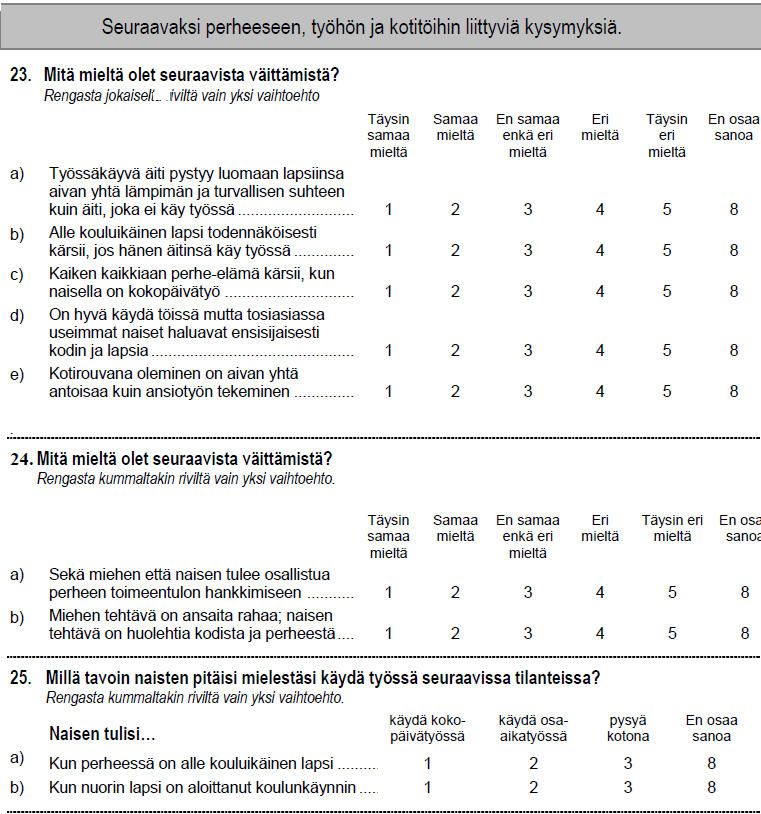
\includegraphics[width=0.5\linewidth]{img/substvar_fi_Q1Q2} 

}

\caption{Suomenkielinen lomake}\label{fig:suom-kys}
\end{figure}

\textbf{taustamuuttujat}

\textbf{k} maa, sukupuoli, haastateltavan ikä, koulutustaso, ``virallinen'' juridinen parisuhdestatus,
pääasiallinen toimi (töissä, eläkkeellä jne), lasten lukumäärä perheessä ja asuinpaikka (maaseutu,
suurkaupunki jne.), oma arvio sosiaalisesta asemasta (1-10). Kysymyksiä, tiedot tosin
kerätty eri tavoin eri maissa.

\textbf{K} Aineistossa mukana puuttuvat vastaukset, puuttuvia ei ole kolmessa muuttujassa
(maa, ikä ja sukupuoli). Muutamilla havainnoilla puuttui tieto iästä tai sukupuolesta,
ja ne rajattiin pois.

Kuvataan tarkemmin, kun käytetään.

\textbf{Miten aineistoa on käytetty?}.

\textbf{Korrespondenssianalyysin esimerkkiaineistona}

Michael Greenacre on käyttänyt aineistoa eri vuosilta luentomateriaaleissa (Helsinki 2017 MCA, viite Moodleen?) ja kahdessa oppikirjassa (\citep{RefWorks:doc:5a857a43e4b0ed2d44664d7c}, \citep{RefWorks:doc:5a857a43e4b0ed2d44664d78}).ISSP - aineisto vuodelta 1989 on käytetty myös neljän ``singuaariarvohajoitelmaan perustuvan menetelmän'' vertailuun\citep{RefWorks:doc:5b6f159ce4b0bc0f31734b76}.

``We consider the joint analysis of two matched matrices which have common
rows and columns, for example multivariate data observed at two time points or split
according to a dichotomous variable. Methods of interest include principal components
analysis for interval-scaled data, correspondence analysis for frequency data, log-ratio
analysis of compositional data and linear biplots in general, all of which depend on the
singular value decomposition. A simple result in matrix algebra shows that by setting up
two matched matrices in a particular block format, matrix sum and difference components
can be analysed using a single application of the singular value decomposition algorithm.
The methodology is applied to data from the International Social Survey Program
comparing male and female attitudes on working wives across eight countries. The resulting
biplots optimally display the overall cross-cultural differences as well as the male--female
differences. The case of more than two matched matrices is also discussed.''

Blasius ja Thiessen (\citep{RefWorks:doc:5b15542ee4b0e2616bc42dca}) arvioivat aineiston laatua ja ja maiden vertailtavuutta vuoden 1994 aineistolla.

``This paper provides empirically-based criteria for selecting Items and countries to develop measures of an underlying construct of interest that are comparable in cross-national research. Using data from the 1994 International Social Survey Program and applying multiple correspondence analysis to a set of common items in each of the 24 participating countries, we show that both the quality of the data, as well as its underlying structure - and therefore meaning - vary considerably between countries. The approach we use for screening countries and items is especially useful in situations where the psychometric properties of the items have not been well established in previous research.''

\textbf{tärkeä rajaus} Substanssitutkimusta ei tässä käsitellä.

``ISSP - saitilla'' löytyy bibliografia, ja hakupalveluillakin voi haravoida.
\textbf{zxy} www.gesis.org - sivustolta löytyy myös \href{https://search.gesis.org/research_data/ZA5900}{julkaisuluettelo}, voiko linkin laittaa alaviitteeksi tai suoraan leipätekstiin?

Sukupuoliroolien (gender roles) ja niihin liittyvien asenteiden vertailevaa kansainvälistä (cross-cultural) tutkimusta on tehty paljon. Tutkimusongelman sisällöllisten ja teoreettisen kysymysten nykytilaa kuvaa Walterin\citep{RefWorks:doc:5bd08fb6e4b05c5447c9a9f9} tuore artikkeli. Omnibus surveys ?

\hypertarget{yksinkertainen-korrespondenssianalyysi}{%
\chapter{Yksinkertainen korrespondenssianalyysi}\label{yksinkertainen-korrespondenssianalyysi}}

\textbf{k1} Yksi kysymys, kuusi maata, peruskäsitteet

\textbf{k2} Luvun tärkeimmät asiat; mitä on luvassa?

\hypertarget{uxe4iti-tuxf6issuxe4}{%
\section{Äiti töissä}\label{uxe4iti-tuxf6issuxe4}}

\textbf{k1}``Alle kouluikäinen lapsi todennäköisesti kärsii, jos hänen äitinsä käy työssä''.
Lyhennän muotoon äiti töissä. ISSP-tutkimuksissa kaksi kysymystä, joissa sana ``äiti'',
MG havainnut ne poikkeaviksi (\textbf{\#V ?}).
\textbf{zxy} Edellisessä luvussa on esitelyt aineisto, ja kerrottu rajaukset.

Tarkistetaan uudet muuttujat (koodilohkon tulostus pois tarvittaessa).

\hypertarget{kahden-muuttujan-frekvenssitaulukon-analyysi}{%
\section{Kahden muuttujan frekvenssitaulukon analyysi}\label{kahden-muuttujan-frekvenssitaulukon-analyysi}}

\textbf{k} Kolme taulukkoa: frekvenssitaulukko, riviprosentit ja sarakeprosentit

\begin{table}

\caption{\label{tab:simpeCA-frekTa1}Kysymyksen Q1b vastaukset maittain}
\centering
\begin{tabular}[t]{lllllll}
\toprule
  & S & s & ? & e & E & Total\\
\midrule
BE & 191 & 451 & 438 & 552 & 381 & 2013\\
BG & 118 & 395 & 205 & 190 & 13 & 921\\
DE & 165 & 375 & 198 & 538 & 438 & 1714\\
DK & 70 & 238 & 152 & 232 & 696 & 1388\\
FI & 47 & 188 & 149 & 423 & 303 & 1110\\
\addlinespace
HU & 219 & 288 & 225 & 190 & 75 & 997\\
Total & 810 & 1935 & 1367 & 2125 & 1906 & 8143\\
\bottomrule
\end{tabular}
\end{table}

\begin{table}

\caption{\label{tab:simpeCA-rprosTa1}Kysymyksen Q1b vastaukset, riviprosentit}
\centering
\begin{tabular}[t]{lllllll}
\toprule
  & S & s & ? & e & E & Total\\
\midrule
BE & 9.49 & 22.40 & 21.76 & 27.42 & 18.93 & 100.00\\
BG & 12.81 & 42.89 & 22.26 & 20.63 & 1.41 & 100.00\\
DE & 9.63 & 21.88 & 11.55 & 31.39 & 25.55 & 100.00\\
DK & 5.04 & 17.15 & 10.95 & 16.71 & 50.14 & 100.00\\
FI & 4.23 & 16.94 & 13.42 & 38.11 & 27.30 & 100.00\\
\addlinespace
HU & 21.97 & 28.89 & 22.57 & 19.06 & 7.52 & 100.00\\
All & 9.95 & 23.76 & 16.79 & 26.10 & 23.41 & 100.00\\
\bottomrule
\end{tabular}
\end{table}

\begin{table}

\caption{\label{tab:simpeCA-cprosTa1}Kysymyksen Q1b vastaukset, sarakeprosentit}
\centering
\begin{tabular}[t]{lllllll}
\toprule
  & S & s & ? & e & E & All\\
\midrule
BE & 23.58 & 23.31 & 32.04 & 25.98 & 19.99 & 24.72\\
BG & 14.57 & 20.41 & 15.00 & 8.94 & 0.68 & 11.31\\
DE & 20.37 & 19.38 & 14.48 & 25.32 & 22.98 & 21.05\\
DK & 8.64 & 12.30 & 11.12 & 10.92 & 36.52 & 17.05\\
FI & 5.80 & 9.72 & 10.90 & 19.91 & 15.90 & 13.63\\
\addlinespace
HU & 27.04 & 14.88 & 16.46 & 8.94 & 3.93 & 12.24\\
Total & 100.00 & 100.00 & 100.00 & 100.00 & 100.00 & 100.00\\
\bottomrule
\end{tabular}
\end{table}

\textbf{k} \textbf{Taulkoista}

Ensimmäinen taulukko on data, lukumäärädataa. Toinen ja kolmas kaksi näkökulmaa
samaan taulukkoon. Sarakkeilla ja riveillä on erilainen rooli, tässä riviprosentit
ovat luonteva tapa verrata ``riippuvaa muuttujaa'', eri maita.

\textbf{k} Rivit on saatu alkuperäisestä aineistosta osajoukkojen summina. MG:n
terminologialla ``samples''.

\textbf{Kuvat}

\begin{figure}
\centering
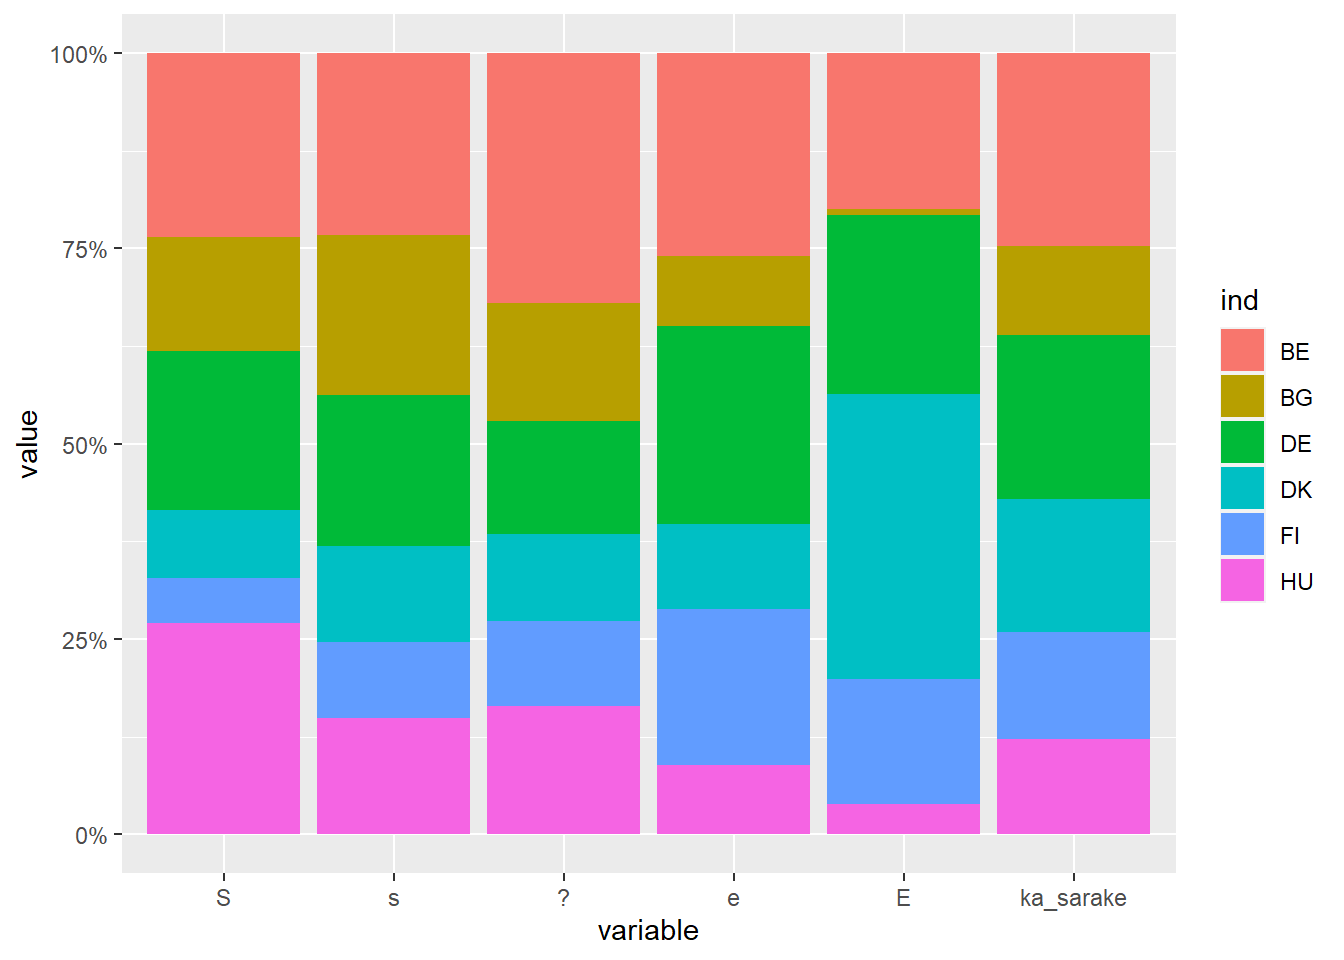
\includegraphics{JH_ca_files/figure-latex/g1-2kuva1-1.pdf}
\caption{\label{fig:g1-2kuva1}Q1b:Sarakeprofiilit ja keskiarvoprofiili}
\end{figure}

\begin{figure}
\centering
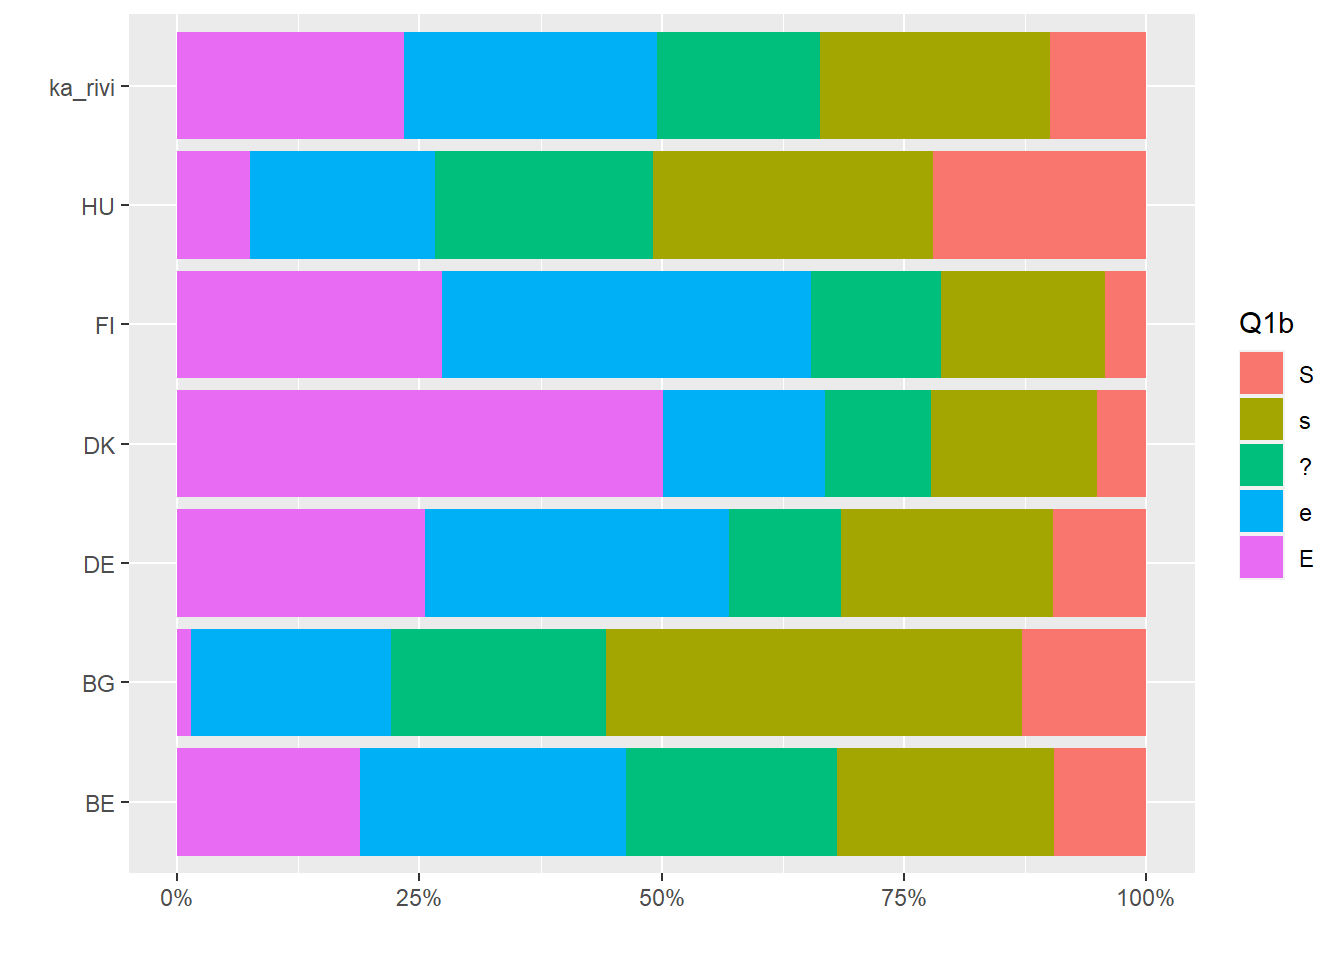
\includegraphics{JH_ca_files/figure-latex/g1-2kuva2-1.pdf}
\caption{\label{fig:g1-2kuva2}Q1b: riviprofiilit ja keskiarvorivi}
\end{figure}

\hypertarget{yksinkertaisen-korrespondenssianalyysi---tulkinnan-syventuxe4minen}{%
\chapter{Yksinkertaisen korrespondenssianalyysi - tulkinnan syventäminen}\label{yksinkertaisen-korrespondenssianalyysi---tulkinnan-syventuxe4minen}}

\textbf{xyz} Tarkasti läpi keskeiset tulokset ja niiden tulkinta, kaavat, ja ytimenä eri kuvat eli kartat.

\hypertarget{yksinkertaisen-korrespondenssianalyysin-laajennuksia}{%
\chapter{Yksinkertaisen korrespondenssianalyysin laajennuksia}\label{yksinkertaisen-korrespondenssianalyysin-laajennuksia}}

\textbf{xyz} Yksinkertainen korrespondenssianalyysi on menetelmän tulkinnan perusta. Perusasetelmaa kahden luokittelumuuttujan ristiintaulukoinnista voidaan laajentaa monipuolisempiin tutkimusasetelmiin. Varsinainen useamman muuttujan korrespondenssianalyysi (MCA - multiple correspondence analysis) esitellään seuraavassa luvussa.

\hypertarget{liitteet}{%
\chapter*{Liitteet}\label{liitteet}}
\addcontentsline{toc}{chapter}{Liitteet}

\hypertarget{suomenkielinen-lomake-esimerkki}{%
\section{Suomenkielinen lomake (esimerkki)}\label{suomenkielinen-lomake-esimerkki}}

Tämä kuva on myös tekstissä, kätevä tapa esittää siististi kysymysten pitkät
versiot.

\begin{Shaded}
\begin{Highlighting}[]
\NormalTok{knitr}\OperatorTok{::}\KeywordTok{include_graphics}\NormalTok{(}\StringTok{'img/substvar_fi_Q1Q2.png'}\NormalTok{)}
\end{Highlighting}
\end{Shaded}

\begin{figure}

{\centering 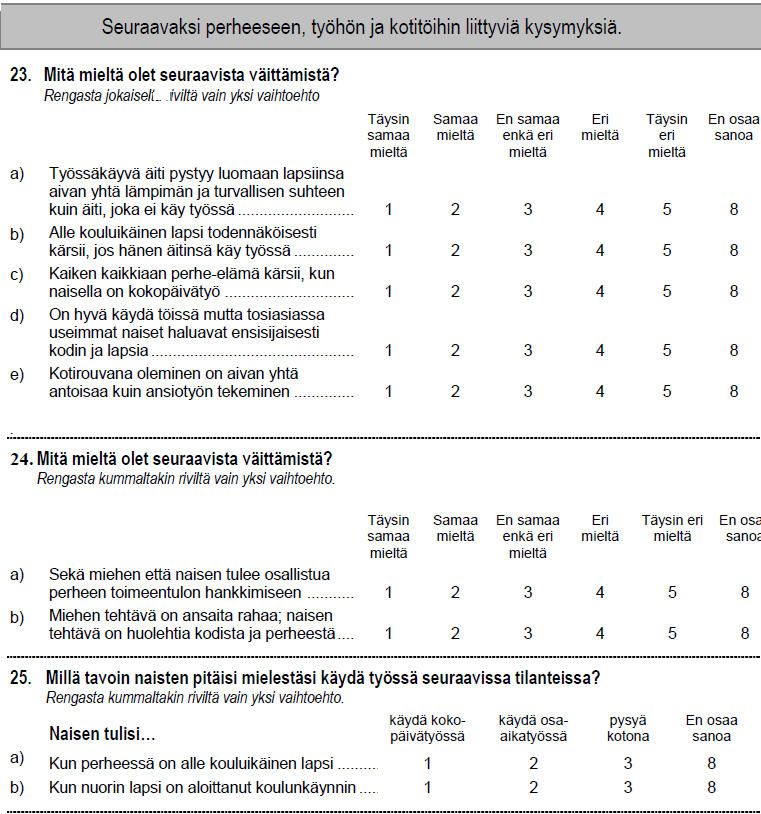
\includegraphics[width=0.6\linewidth]{img/substvar_fi_Q1Q2} 

}

\caption{Esimerkki suomenkielisestä lomakkeesta}\label{fig:L1suomlom1}
\end{figure}

\hypertarget{r---koodi}{%
\section{R - koodi}\label{r---koodi}}

\begin{Shaded}
\begin{Highlighting}[]
\CommentTok{# 18.10.2020}
\KeywordTok{library}\NormalTok{(rgl)}
\KeywordTok{library}\NormalTok{(ca)}
\KeywordTok{library}\NormalTok{(haven)}
\KeywordTok{library}\NormalTok{(dplyr)}
\KeywordTok{library}\NormalTok{(knitr)}
\KeywordTok{library}\NormalTok{(tidyverse)}
\KeywordTok{library}\NormalTok{(lubridate)}
\KeywordTok{library}\NormalTok{(rmarkdown)}
\KeywordTok{library}\NormalTok{(ggplot2)}
\KeywordTok{library}\NormalTok{(furniture)}
\KeywordTok{library}\NormalTok{(scales) }\CommentTok{# G_1_2 - kuva}
\KeywordTok{library}\NormalTok{(reshape2)  }\CommentTok{# G_1_2 - kuva}
\KeywordTok{library}\NormalTok{(printr) }\CommentTok{#19.5.18 taulukoiden ja matriisien tulostukseen}
\KeywordTok{library}\NormalTok{(bookdown)}
\KeywordTok{library}\NormalTok{(tinytex)}
\KeywordTok{library}\NormalTok{(assertthat)}


\CommentTok{# automatically create a bib database for R packages}
\NormalTok{knitr}\OperatorTok{::}\KeywordTok{write_bib}\NormalTok{(}\KeywordTok{c}\NormalTok{(}
  \KeywordTok{.packages}\NormalTok{(), }\StringTok{'bookdown'}\NormalTok{, }\StringTok{'knitr'}\NormalTok{, }\StringTok{'rmarkdown'}
\NormalTok{), }\StringTok{'packages.bib'}\NormalTok{)}

\CommentTok{# include FALSE: ei koodia eikä tulostusta dokumenttiin - poistettava turhia}
\CommentTok{# välitulostuksia (18.10.2020)}
\CommentTok{# Aineiston rajaamisen kolme vaihetta (10.2018)}
\CommentTok{# }
\CommentTok{# TIEDOSTOJEN NIMEÄMINEN}
\CommentTok{#}
\CommentTok{# R-datatiedostot .data - tarkenteella ovat osajoukkoja koko ISSP-datasta ISSP2012.data}
\CommentTok{# R-datatiedostot .dat - tarkenteella: mukana alkuperäisten muuttujien muunnoksia }
\CommentTok{# (yleensä as_factor), alkuperäisissä muuttujissa mukana SPSS-tiedoston metadata.}
\CommentTok{#}
\CommentTok{# Luokittelumuuttujan tyyppi on datan lukemisen jälkeen yleensä merkkijono (char) }
\CommentTok{# ja haven_labelled. }
\CommentTok{#}
\CommentTok{# Muutetaan R-datassa ordinaali- tai  nominaaliasteikon muuttujat haven-paketin }
\CommentTok{# as_factor - funktiolla faktoreiksi. R:n faktorityypin muuttujille voidaan tarvittaessa }
\CommentTok{# määritellä järjestys, toistaiseksi niin ei tehdä (25.9.2018). }
\CommentTok{#}
\CommentTok{# Muunnetun muuttujan rinnalla säilytetään SPSS-tiedostosta luettu muuttja, metatiedot säilyvät }
\CommentTok{# alkuperäisessä.}
\CommentTok{#       }
\CommentTok{# R-datatiedostot joiden nimen loppuosa on muotoa *esim1.dat: käytetään analyyseissä}
\CommentTok{#}
\CommentTok{# 1. VALITAAN MAAT (25) -> ISSP2012jh1a.data. Muuttujat koodilohkossa datasel_vars1}
\CommentTok{#}
\CommentTok{# kolme maa-muuttujaa datassa. V3 erottelee joidenkin maiden alueita, V4 on koko }
\CommentTok{# maan koodi ja C_ALPHAN on maan kaksimerkkinen tunnus.}
\CommentTok{#}
\CommentTok{# V3 - Country/ Sample ISO 3166 Code (see V4 for codes for whole nation states)}
\CommentTok{# V3 erot valituissa maissa}
\CommentTok{# 5601 BE-FLA-Belgium/ Flanders}
\CommentTok{# 5602 BE-WAL-Belgium/ Wallonia}
\CommentTok{# 5603 BE-BRU-Belgium/ Brussels}
\CommentTok{# 27601 DE-W-Germany-West}
\CommentTok{# 27602 DE-E-Germany-East}
\CommentTok{# 62001 PT-Portugal 2012: first fieldwork round (main sample)}
\CommentTok{# 62002 PT-Portugal 2012: second fieldwork round (complementary sample)}
\CommentTok{# Myös tämä on erikoinen, näyttää olevan vakio kun V4 = 826:}
\CommentTok{# 82601 GB-GBN-Great Britain}
\CommentTok{# Portugalissa ainestoa täydennettiin, koska siinä oli puutteita. Jako ei siis ole oleellinen,}
\CommentTok{# mutta muuut ovat. Tähdellä merkityt maat valitaan johdattelevaan esimerkkiin.}
\CommentTok{#}
\CommentTok{# Maat (25)}
\CommentTok{#}
\CommentTok{# 36 AU-Australia}
\CommentTok{# 40 AT-Austria}
\CommentTok{# 56 BE-Belgium*}
\CommentTok{# 100 BG-Bulgaria*}
\CommentTok{# 124 CA-Canada}
\CommentTok{# 191 HR-Croatia}
\CommentTok{# 203 CZ-Czech Republic}
\CommentTok{# 208 DK-Denmark*}
\CommentTok{# 246 FI-Finland*}
\CommentTok{# 250 FR-France}
\CommentTok{# 276 DE-Germany*}
\CommentTok{# 348 HU-Hungary*}
\CommentTok{# 352 IS-Iceland}
\CommentTok{# 372 IE-Ireland}
\CommentTok{# 428 LV-Latvia}
\CommentTok{# 440 LT-Lithuania}
\CommentTok{# 528 NL-Netherlands}
\CommentTok{# 578 NO-Norway}
\CommentTok{# 616 PL-Poland}
\CommentTok{# 620 PT-Portugal}
\CommentTok{# 643 RU-Russia}
\CommentTok{# 703 SK-Slovakia}
\CommentTok{# 705 SI-Slovenia}
\CommentTok{# 752 SE-Sweden}
\CommentTok{# 756 CH-Switzerland}
\CommentTok{# 826 GB-Great Britain and/or United Kingdom - jätetään pois jotta saadaan TOPBOT }
\CommentTok{#                          -muuttuja mukaan (top-bottom self-placement) .(9.10.18)}
\CommentTok{# 840 US-United States - jätetään pois, jotta saadaan TOPBOT-muuttuja mukaan.(10.10.18)}
\CommentTok{#}
\CommentTok{# Belgian ja Saksan alueet:}
\CommentTok{#  V3}
\CommentTok{#  5601     BE-FLA-Belgium/ Flanders}
\CommentTok{#  5602     BE-WAL-Belgium/ Wallonia}
\CommentTok{#  5603     BE-BRU-Belgium/ Brussels}
\CommentTok{# 27601     DE-W-Germany-West}
\CommentTok{# 27602     DE-E-Germany-East}
\CommentTok{#}
\CommentTok{# Unkari (348) toistaiseksi mukana, mutta joissain kysymyksissä myös Unkarilla on }
\CommentTok{# poikkeavia vastausvaihtoehtoja(HU_V18, HU_V19,HU_V20). Jos näitä muuttujia käytetään, }
\CommentTok{# Unkari on parempi jättää pois. }
\CommentTok{# }
\CommentTok{#}
\CommentTok{# (25.4.2018) user_na  }
\CommentTok{# haven-paketin read_spss - funktiolla voi r-tiedostoon lukea myös SPSS:n sallimat kolme }
\CommentTok{# (yleensä 7, 8, 9) tarkempaa koodia puuttuvalle tiedolle.}
\CommentTok{# "If TRUE variables with user defined missing will be read into labelled_spss objects. }
\CommentTok{# If FALSE, the default, user-defined missings will be converted to NA"}
\CommentTok{# https://www.rdocumentation.org/packages/haven/versions/1.1.0/topics/read_spss}
\CommentTok{#}
 
\NormalTok{ISSP2012jh.data <-}\StringTok{ }\KeywordTok{read_spss}\NormalTok{(}\StringTok{"data/ZA5900_v4-0-0.sav"}\NormalTok{) }\CommentTok{#luetaan alkuperäinen data R- dataksi (df).}

\CommentTok{#str(ISSP2012jh.data)}

\NormalTok{incl_countries25 <-}\StringTok{ }\KeywordTok{c}\NormalTok{(}\DecValTok{36}\NormalTok{, }\DecValTok{40}\NormalTok{, }\DecValTok{56}\NormalTok{,}\DecValTok{100}\NormalTok{, }\DecValTok{124}\NormalTok{, }\DecValTok{191}\NormalTok{, }\DecValTok{203}\NormalTok{, }\DecValTok{208}\NormalTok{, }\DecValTok{246}\NormalTok{, }\DecValTok{250}\NormalTok{, }\DecValTok{276}\NormalTok{, }\DecValTok{348}\NormalTok{, }\DecValTok{352}\NormalTok{, }
                      \DecValTok{372}\NormalTok{, }\DecValTok{428}\NormalTok{, }\DecValTok{440}\NormalTok{, }\DecValTok{528}\NormalTok{, }\DecValTok{578}\NormalTok{, }\DecValTok{616}\NormalTok{, }\DecValTok{620}\NormalTok{, }\DecValTok{643}\NormalTok{, }\DecValTok{703}\NormalTok{, }\DecValTok{705}\NormalTok{, }\DecValTok{752}\NormalTok{, }\DecValTok{756}\NormalTok{)}

\CommentTok{#str(ISSP2012jh.data)}
\CommentTok{#str(ISSP2012jh.data) #61754 obs. of  420 variables - kaikki}

\NormalTok{ISSP2012jh1a.data <-}\StringTok{ }\KeywordTok{filter}\NormalTok{(ISSP2012jh.data, V4 }\OperatorTok\StringTok{ }\NormalTok{incl_countries25)}

\CommentTok{#head(ISSP2012jh1a.data)}
\CommentTok{#str(ISSP2012jh1a.data) #34271 obs. of  420 variables, Espanja ja Iso-Britannia}
\CommentTok{#                       pois (9.10.2018)}
\CommentTok{# str(ISSP2012jh1a.data) # 32969 obs. of  420 variable, Espanja Iso-Britannia, }
\CommentTok{#                        USA pois (10.10.2018)}
\CommentTok{#}
\CommentTok{# names() # muuttujen nimet}
\CommentTok{# Maakohtaiset muuttujat (kun on poikettu ISSP2012 - vastausvaihtoehdoista tms.) }
\CommentTok{# on aineistossa eroteltu maatunnus-etuliitteellä (esimerkiksi ES_V7).}
\CommentTok{# Demografisissa ja muissa taustamuuttujissa suuri osa tiedoista on kerätty maa-}
\CommentTok{# kohtaisilla lomakkeilla. Vertailukelpoiset muuttujat on konstruoitu niistä.}
\CommentTok{# Muuttujia on 420, vain osa yhteisiä kaikille maille.}

\CommentTok{# include FALSE: ei koodia eikä tulostusta dokumenttiin - poistettava turhia}
\CommentTok{# välitulostuksia (18.10.2020)}
\CommentTok{# 2. VALITAAN MUUTTUJAT  -> ISSP2012jh1b.data. Maat valittu koodilohkossa datasel_country1}
\CommentTok{#}
\CommentTok{#}
\CommentTok{# Muuttujat on luokiteltu dokumentissa ZA5900_overview.pdf}
\CommentTok{# https://zacat.gesis.org/webview/index.jsp?object=http://zacat.gesis.org/obj/fStudy/ZA5900}
\CommentTok{# Study Description -> Other Study Description -> Related Materials}
\CommentTok{# }
\CommentTok{#}

\CommentTok{# METADATA}

\NormalTok{metavars1 <-}\StringTok{ }\KeywordTok{c}\NormalTok{(}\StringTok{"V1"}\NormalTok{, }\StringTok{"V2"}\NormalTok{, }\StringTok{"DOI"}\NormalTok{)}

\CommentTok{#MAA - maakoodit ja maan kahden merkin tunnus}

\NormalTok{countryvars1 <-}\StringTok{ }\KeywordTok{c}\NormalTok{(}\StringTok{"V3"}\NormalTok{,}\StringTok{"V4"}\NormalTok{,}\StringTok{"C_ALPHAN"}\NormalTok{)}

\CommentTok{# SUBSTANSSIMUUTTUJAT - Attitudes towards family and gender roles (9)}
\CommentTok{#}
\CommentTok{# Yhdeksän kysymystä (lyhennetyt versiot, englanniksi), vastausvaihtoehdot Q1-Q2}
\CommentTok{#}
\CommentTok{# 1 = täysin samaa mieltä, 2 = samaa mieltä, 3 = ei samaa eikä eri mieltä, }
\CommentTok{# 4 = eri mieltä, 5 = täysin eri mieltä}
\CommentTok{# }
\CommentTok{# Q1a Working mother can have warm relation with child}
\CommentTok{# Q1b Pre-school child suffers through working mother}
\CommentTok{# Q1c Family life suffers through working mother}
\CommentTok{# Q1d Women’s preference: home and children}
\CommentTok{# Q1e Being housewife is satisfying}
\CommentTok{#}
\CommentTok{# Q2a Both should contribute to household income}
\CommentTok{# Q2b Men’s job is earn money, women’s job household}
\CommentTok{#}
\CommentTok{# Q3a Should women work: Child under school age }
\CommentTok{# Q3b Should women work: Youngest kid at school}
\CommentTok{# 1= kokopäivätyö, 2 = osa-aikatyö, 3 = pysyä kotona, 8 = en osaa sanoa (can't choose), 9 = no answer}
\CommentTok{#}
\CommentTok{# Kysymysten Q3a ja Q3b eos-vastaus ei ole sama kuin "en samaa enkä eri  mieltä" (ns. neutraali }
\CommentTok{# vaihtoehto), mutta kieltäytymisiä jne. (koodi 9) on aika vähän. Kolmessa }
\CommentTok{# maassa ne on yhdistety: }
\CommentTok{# (8 Can't choose, CA:can't choose+no answer, KR:don't know+refused, NL:don't know).}
\CommentTok{# Kun SPSS-tiedostosta ei ole tuotu puuttuvan tiedon tarkempaa luokittelua,}
\CommentTok{# erottelua ei voi tehdä.}
\CommentTok{#}
\CommentTok{# }
\CommentTok{#}

\NormalTok{substvars1 <-}\StringTok{ }\KeywordTok{c}\NormalTok{(}\StringTok{"V5"}\NormalTok{,}\StringTok{"V6"}\NormalTok{,}\StringTok{"V7"}\NormalTok{,}\StringTok{"V8"}\NormalTok{,}\StringTok{"V9"}\NormalTok{,}\StringTok{"V10"}\NormalTok{,}\StringTok{"V11"}\NormalTok{,}\StringTok{"V12"}\NormalTok{,}\StringTok{"V13"}\NormalTok{) }\CommentTok{# 9 muuttujaa}

\CommentTok{# Nämä yhteiset muuttujat pois (maaspesifien muuttujien lisäksi) :}
\CommentTok{#}
\CommentTok{# "V14","V15","V16",  "V17","V18","HU_V18","V19","HU_V19","V20","HU_V20","V21",}
\CommentTok{# "V28","V29","V30","V31","V32","V33",# "V34", "V35", "V36", "V37", "V38", "V39",}
\CommentTok{# "V40", "V41", "V42", "V43", "V44", "V45", "V46", "V47", "V48", "V49", "V50", }
\CommentTok{# "V51", "V52", "V53", "V54", "V55", "V56", "V57", "V58", "V59", "V60", "V61", }
\CommentTok{# "V62", "V63", "V64", "V65", "V65a","V66", "V67"}
\CommentTok{#}
\CommentTok{#}
\CommentTok{# DEMOGRAFISET JA MUUT TAUSTAMUUTTUJAT (8)}
\CommentTok{#}
\CommentTok{# AGE, SEX}
\CommentTok{#}
\CommentTok{# DEGREE - Highest completed degree of education: Categories for international comparison. }
\CommentTok{# Slightly re-arranged subset of ISCED-97}
\CommentTok{#}
\CommentTok{# 0 No formal education}
\CommentTok{# 1 Primary school (elementary school)}
\CommentTok{# 2 Lower secondary (secondary completed does not allow entry to university: obligatory school)}
\CommentTok{# 3 Upper secondary (programs that allow entry to university or programs that allow to entry }
\CommentTok{#   other ISCED level 3 programs - designed to prepare students for direct entry into the labour market)}
\CommentTok{# 4 Post secondary, non-tertiary (other upper secondary programs toward labour market or technical formation)}
\CommentTok{# 5 Lower level tertiary, first stage (also technical schools at a tertiary level)}
\CommentTok{# 6 Upper level tertiary (Master, Dr.)}
\CommentTok{# 9 No answer, CH: don't know}
\CommentTok{# Yhdistelyt?}
\CommentTok{#}
\CommentTok{# MAINSTAT - main status: Which of the following best describes your current situation?}
\CommentTok{#}
\CommentTok{# 1 In paid work}
\CommentTok{# 2 Unemployed and looking for a job, HR: incl never had a job}
\CommentTok{# 3 In education}
\CommentTok{# 4 Apprentice or trainee}
\CommentTok{# 5 Permanently sick or disabled}
\CommentTok{# 6 Retired}
\CommentTok{# 7 Domestic work}
\CommentTok{# 8 In compulsory military service or community service}
\CommentTok{# 9 Other}
\CommentTok{# 99 No answer}
\CommentTok{# Armeijassa tai yhdyskuntapalvelussa muutamia, muutamissa maissa.Kategoriassa 9 }
\CommentTok{# on hieman väkeä. Yhdistetään 8 ja 9. Huom! Esim Puolassa ei yhtään eläkeläistä}
\CommentTok{# eikä kategoriaa 9, Saksassa ei ketään kategoriassa 9.}
\CommentTok{#}
\CommentTok{# TOPBOT - Top-Bottom self-placement (10 pt scale)}
\CommentTok{#}
\CommentTok{# "In our society, there are groups which tend to be towards the top and groups }
\CommentTok{# which tend to be towards the bottom. Below is a scale that runs}
\CommentTok{# from the top to the bottom. Where would you put yourself on this scale?"}
\CommentTok{# Eri maissa hieman erilaisia kysymyksiä. }
\CommentTok{#}
\CommentTok{# HHCHILDR - How many children in household: children between [school age] and}
\CommentTok{# 17 years of age}
\CommentTok{#}
\CommentTok{# 0 No children}
\CommentTok{# 1 One child}
\CommentTok{# 2 2 children}
\CommentTok{# 21 21 children}
\CommentTok{# 96 NAP (Code 0 in HOMPOP)}
\CommentTok{# 97 Refused}
\CommentTok{# 99 No answer}
\CommentTok{#}
\CommentTok{# Voisi koodata dummymuuttujaksi lapsia (1) - ei lapsia (0).}
\CommentTok{# Ranskan datassa on erittäin iso osa puuttuvia tietoja ( "99"", n. 20 %), myös }
\CommentTok{# Austarlialla aika paljon. Sama tilanne myös muissa perheen kokoon liittyvissä }
\CommentTok{# kysymyksissä.}
\CommentTok{#}
\CommentTok{# MARITAL - Legal partnership status }
\CommentTok{#}
\CommentTok{# What is your current legal marital status?}
\CommentTok{# The aim of this variable is to measure the current 'legal' marital status '. }
\CommentTok{# PARTLIV - muuttujassa on 'de facto' - tilanteen tieto parisuhteesta}
\CommentTok{#}
\CommentTok{# 1 Married}
\CommentTok{# 2 Civil partnership}
\CommentTok{# 3 Separated from spouse/ civil partner (still legally married/ still legally }
\CommentTok{#   in a civil partnership)}
\CommentTok{# 4 Divorced from spouse/ legally separated from civil partner}
\CommentTok{# 5 Widowed/ civil partner died}
\CommentTok{# 6 Never married/ never in a civil partnership, single}
\CommentTok{# 7 Refused}
\CommentTok{# 8 Don't know}
\CommentTok{# 9 No answer}
\CommentTok{#}
\CommentTok{# URBRURAL - Place of living: urban - rural}
\CommentTok{#}
\CommentTok{# 1 A big city}
\CommentTok{# 2 The suburbs or outskirts of a big city}
\CommentTok{# 3 A town or a small city}
\CommentTok{# 4 A country village}
\CommentTok{# 5 A farm or home in the country}
\CommentTok{# 7 Other answer}
\CommentTok{# 9 No answer}
\CommentTok{# 1 ja 2 vaihtelevat aika paljon maittain, parempi laskea yhteen. Unkarista puuttuu }
\CommentTok{# jostain syystä kokonaan vaihtoehto 5.  Vaihotehdon 7 on valinnut vain 4 vastaajaa Ranskasta.}
\CommentTok{# Yhdistetään 1 ja 2 = city, 3 = town, rural= 4, 5, 7}
\CommentTok{#}

\NormalTok{bgvars1 <-}\StringTok{ }\KeywordTok{c}\NormalTok{( }\StringTok{"SEX"}\NormalTok{,}\StringTok{"AGE"}\NormalTok{,}\StringTok{"DEGREE"}\NormalTok{, }\StringTok{"MAINSTAT"}\NormalTok{, }\StringTok{"TOPBOT"}\NormalTok{, }\StringTok{"HHCHILDR"}\NormalTok{, }\StringTok{"MARITAL"}\NormalTok{, }\StringTok{"URBRURAL"}\NormalTok{)}

\CommentTok{#Valitaan muuttujat}

\NormalTok{jhvars1 <-}\StringTok{ }\KeywordTok{c}\NormalTok{(metavars1,countryvars1, substvars1,bgvars1)}

\CommentTok{#jhvars1}
\NormalTok{ISSP2012jh1b.data <-}\StringTok{ }\KeywordTok{select}\NormalTok{(ISSP2012jh1a.data, }\KeywordTok{all_of}\NormalTok{(jhvars1)) }

\CommentTok{# laaja aineisto - mukana havainnot joissa puuttuvia tietoja}
\CommentTok{# hauska detalji URBRURAL - muuttujan metatiedoissa viite jonkun työaseman hakemistoon}
\CommentTok{# str(ISSP2012jh1b.data) #32969 obs. of  23 variables }
\CommentTok{# }
\CommentTok{# SUBSTANSSIMUUTTUJAT}
\CommentTok{#}
\CommentTok{# $ V5      : 'haven_labelled' num  5 1 2 2 1 NA 2 4 2 2 ...}
\CommentTok{#  ..- attr(*, "label")= chr "Q1a Working mom: warm relationship with children as a not working mom"}
\CommentTok{#  ..- attr(*, "labels")= Named num  0 1 2 3 4 5 8 9}
\CommentTok{#}
\CommentTok{# ISSP2012jh1b.data$V5 näyttää tarkemmin rakenteen}
\CommentTok{#}
\CommentTok{# glimpse(ISSP2012jh1b.data)}
\CommentTok{# str(ISSP2012jh1b.data) # 32969 obs. of  23 variables}

\CommentTok{# Poistetaan havainnot, joissa ikä (AGE) tai sukupuolitieto puuttuu (5.7.2019)}

\NormalTok{ISSP2012jh1c.data <-}\StringTok{ }\KeywordTok{filter}\NormalTok{(ISSP2012jh1b.data, (}\OperatorTok{!}\KeywordTok{is.na}\NormalTok{(SEX) }\OperatorTok{&}\StringTok{ }\OperatorTok{!}\KeywordTok{is.na}\NormalTok{(AGE)))}

\KeywordTok{str}\NormalTok{(ISSP2012jh1c.data) }\CommentTok{# 32823 obs. of  23 variables, 32969-32823 = 146}
\CommentTok{# TARKISTUS 8.6.20 dplyr 1.0.0-päivitys: havaintojen ja muuttujien määrä ok.}

\CommentTok{# VAIHE 1 - muuttujat joissa ei ole puuttuvia tietoja}

\CommentTok{# vaihe 1.1 haven_labelled ja chr -> as_factor}

\NormalTok{ISSP2012jh1d.dat <-}\StringTok{ }\NormalTok{ISSP2012jh1c.data }\OperatorTok
\StringTok{    }\KeywordTok{mutate}\NormalTok{(}\DataTypeTok{maa =} \KeywordTok{as_factor}\NormalTok{(C_ALPHAN), }\CommentTok{# ei puuttuvia, ei tyhjiä leveleitä}
           \DataTypeTok{maa3 =} \KeywordTok{as_factor}\NormalTok{(V3),  }\CommentTok{# maakoodi, jossa aluejako joillan mailla}
           \DataTypeTok{sp1 =} \KeywordTok{as_factor}\NormalTok{(SEX), }\CommentTok{# ei puuttuvia, tyhjä level "no answer" 999}
\NormalTok{         )}


\CommentTok{# C_ALPHAN - maa - maa3 tarkistuksia}

\CommentTok{# V3}
\CommentTok{# "Pulma" on järjestys. C_ALPHAN ("chr") on aakkosjärjestyksessä, kun luodaan}
\CommentTok{# maa = as_factor(C_ALPHAN) järjestys muuttuu (esiintymisjärjestys datassa?)}
\CommentTok{# maa3 muunnetaan maakoodista (haven_labelled' num), jonka}

\CommentTok{# str(ISSP2012jh1d.dat$maa) #Country Prefix ISO 3166 Code - alphanumeric}
\CommentTok{# attributes(ISSP2012jh1d.dat$maa) # ei tyhiä levels-arvoja, 25 levels}
\CommentTok{# ISSP2012jh1d.dat$maa %>% fct_unique()}
\CommentTok{# ISSP2012jh1d.dat$maa %>% fct_count() # summary kertoo samat tiedot (20.2.20)}
\CommentTok{# sum(is.na(ISSP2012jh1d.dat$maa)) # ei puuttuvia tietoja}
\CommentTok{# ISSP2012jh1d.dat$maa %>% summary() # mukana vain valitut 25 maata}

\CommentTok{# str(ISSP2012jh1d.dat$maa3)  #"Country/ Sample ISO 3166 Code}
                            \CommentTok{#(see V4 for codes for whole nation states)"}
                            \CommentTok{# 29 levels}
\CommentTok{# str(ISSP2012jh1d.dat$V3)}

\CommentTok{# attributes(ISSP2012jh1d.dat$maa3) # ei tyhiä levels-arvoja, 29 levels}
\CommentTok{# sum(is.na(ISSP2012jh1d.dat$maa3)) # nolla ei ole puuttuva tieto! (3.2.20)}
\CommentTok{# ISSP2012jh1d.dat$maa3 %>% fct_unique()}
\CommentTok{# ISSP2012jh1d.dat$maa3 %>% fct_count()}
\CommentTok{# Vain näissä on jaettu maan havainnot (3.2.20)}
\CommentTok{#}
\CommentTok{# [38] BE-FLA-Belgium/ Flanders}
\CommentTok{# [39] BE-WAL-Belgium/ Wallonia}
\CommentTok{# [40] BE-BRU-Belgium/ Brussels}
\CommentTok{# [41] DE-W-Germany-West}
\CommentTok{# [42] DE-E-Germany-East}
\CommentTok{# [43] PT-Portugal 2012: first fieldwork round (main sample)}
\CommentTok{# [44] PT-Portugal 2012: second fieldwork round (complementary sample)}

\CommentTok{# ISSP2012jh1d.dat$maa3 %>% fct_count() #miksi ei tulosta mitään? (3.2.2020)}

\CommentTok{# ISSP2012jh1d.dat$maa3 %>% summary()}
\CommentTok{# ISSP2012jh1d.dat$maa3 %>% fct_unique()}
\CommentTok{# maa3: 25 maata, havaintojen määrä. Poisjätetyissä havaintoja 0.}
\CommentTok{# glimpse(ISSP2012jh1d.dat$maa3)}
\CommentTok{# head(ISSP2012jh1d.dat$maa3)}
\CommentTok{# length(levels(ISSP2012jh1d.dat$maa3))}

\CommentTok{# C_ALPHAN alkuperäinen järjestys, maa aakkosjärjestyssä  (2.2.20)}
\CommentTok{#}
\CommentTok{# Huom1: Myös merkkijonomuuttujaa C_ALPHAN tarvitaan jatkossa.}
\CommentTok{#}
\CommentTok{# Huom2: kun dataa rajataan, on tarkistettava ja tarvittaessa poistettava}
\CommentTok{# "tyhjät" R-factor - muuttujan "maa" luokat (3.2.2020)}


\CommentTok{# vaihe 1.2 tyhjät luokat (levels) pois faktoreista}

\NormalTok{ISSP2012jh1d.dat <-}\StringTok{ }\NormalTok{ISSP2012jh1d.dat }\OperatorTok
\StringTok{    }\KeywordTok{mutate}\NormalTok{(}\DataTypeTok{sp =} \KeywordTok{fct_drop}\NormalTok{(sp1),}
           \DataTypeTok{maa3 =} \KeywordTok{fct_drop}\NormalTok{(maa3)}
\NormalTok{           )}

\CommentTok{#  maa3 - tarkistuksia}

\CommentTok{# str(ISSP2012jh1d.dat$maa3)  # 29 levels}
\CommentTok{# attributes(ISSP2012jh1d.dat$maa3)}
\CommentTok{#sum(is.na(ISSP2012jh1d.dat$maa3)) # nolla ei ole puuttuva tieto! (3.2.20)}
\CommentTok{# ISSP2012jh1d.dat$maa3 %>% summary()}
\CommentTok{# ISSP2012jh1d.dat$maa3 %>% fct_unique()}
\CommentTok{# ISSP2012jh1d.dat$maa3 %>% fct_count()}
\CommentTok{#}
\CommentTok{# str(ISSP2012jh1d.dat$C_ALPHAN)}
\CommentTok{# attributes(ISSP2012jh1d.dat$C_ALPHAN)}

\CommentTok{# TESTAUKSIA}
\CommentTok{# }
\CommentTok{# ISSP2012jh1d.dat %>% tableX(C_ALPHAN, maa)}
\CommentTok{# ISSP2012jh1d.dat %>% tableX(C_ALPHAN, maa3)}
\CommentTok{# ISSP2012jh1d.dat %>% tableX(maa, maa3)}
\CommentTok{# ISSP2012jh1d.dat %>% tableX(V3, maa3)}

\CommentTok{# sp, sp1, SEX - tarkistuksia}
\CommentTok{# }
\CommentTok{# ISSP2012jh1d.dat$sp %>% fct_count()}
\CommentTok{# ISSP2012jh1d.dat$sp %>% fct_count()}
\CommentTok{# ISSP2012jh1d.dat %>% tableX(SEX,sp1)}
\CommentTok{# ISSP2012jh1d.dat %>% tableX(SEX,sp)}
\CommentTok{# ISSP2012jh1d.dat %>% tableX(sp1,sp)}

\CommentTok{# vaihe 1.3 uudet "faktorilabelit"}
\NormalTok{ISSP2012jh1d.dat <-}\StringTok{ }\NormalTok{ISSP2012jh1d.dat }\OperatorTok
\StringTok{    }\KeywordTok{mutate}\NormalTok{(}\DataTypeTok{sp =}
          \KeywordTok{fct_recode}\NormalTok{(sp,}
            \StringTok{"m"}\NormalTok{ =}\StringTok{ "Male"}\NormalTok{,}
            \StringTok{"f"}\NormalTok{ =}\StringTok{ "Female"}\NormalTok{)}
\NormalTok{            )}

\CommentTok{# Tarkistuksia}

\CommentTok{# ISSP2012jh1d.dat$sp %>% fct_unique()}
\CommentTok{# ISSP2012jh1d.dat$sp %>% fct_count()}
\CommentTok{# ISSP2012jh1d.dat$sp %>% summary()}

\CommentTok{# AGE -> ika}
\NormalTok{ISSP2012jh1d.dat}\OperatorTok{$}\NormalTok{ika <-}\StringTok{ }\NormalTok{ISSP2012jh1d.dat}\OperatorTok{$}\NormalTok{AGE}

\CommentTok{# Tarkistuksia}
\KeywordTok{attributes}\NormalTok{(ISSP2012jh1d.dat}\OperatorTok{$}\NormalTok{ika) }\CommentTok{# tyhjä level "No answer"}
\CommentTok{# str(ISSP2012jh1d.dat$ika)}
\NormalTok{ISSP2012jh1d.dat}\OperatorTok{$}\NormalTok{ika }\OperatorTok\StringTok{ }\KeywordTok{summary}\NormalTok{()}

\NormalTok{ISSP2012jh1d.dat }\OperatorTok
\KeywordTok{tableC}\NormalTok{(AGE, ika,}\DataTypeTok{cor_type =} \StringTok{"pearson"}\NormalTok{, }\DataTypeTok{na.rm =} \OtherTok{FALSE}\NormalTok{, }\DataTypeTok{rounding =} \DecValTok{5}\NormalTok{,}
       \DataTypeTok{output =} \StringTok{"text"}\NormalTok{, }\DataTypeTok{booktabs =} \OtherTok{TRUE}\NormalTok{, }\DataTypeTok{caption =} \OtherTok{NULL}\NormalTok{, }\DataTypeTok{align =} \OtherTok{NULL}\NormalTok{,}
       \DataTypeTok{float =} \StringTok{"htb"}\NormalTok{) }\OperatorTok\StringTok{ }\KeywordTok{kable}\NormalTok{()}

\CommentTok{# Ikäjakauma - ei tarvita (18.10.2020)}
\CommentTok{#}
\CommentTok{# ISSP2012jh1d.dat$ika %>% hist(main = "ISSP 2012: vastaajan ikä")}

\CommentTok{# Substanssi- ja taustamuuttujat R-faktoreiksi}
\NormalTok{ISSP2012jh1d.dat <-}\StringTok{ }\NormalTok{ISSP2012jh1d.dat }\OperatorTok
\StringTok{    }\KeywordTok{mutate}\NormalTok{(}\DataTypeTok{Q1a1 =} \KeywordTok{as_factor}\NormalTok{(V5), }\CommentTok{#labels}
            \DataTypeTok{Q1b1 =} \KeywordTok{as_factor}\NormalTok{(V6),}
            \DataTypeTok{Q1c1 =} \KeywordTok{as_factor}\NormalTok{(V7),}
            \DataTypeTok{Q1d1 =} \KeywordTok{as_factor}\NormalTok{(V8),}
            \DataTypeTok{Q1e1 =} \KeywordTok{as_factor}\NormalTok{(V9),}
            \DataTypeTok{Q2a1 =} \KeywordTok{as_factor}\NormalTok{(V10),}
            \DataTypeTok{Q2b1 =} \KeywordTok{as_factor}\NormalTok{(V11),}
            \DataTypeTok{Q3a1 =} \KeywordTok{as_factor}\NormalTok{(V12), }\CommentTok{#labels = vastQ3_labels (W,w,H)}
            \DataTypeTok{Q3b1 =} \KeywordTok{as_factor}\NormalTok{(V13), }\CommentTok{#labels = vastQ3_labels}
            \DataTypeTok{edu1 =} \KeywordTok{as_factor}\NormalTok{(DEGREE),}
            \DataTypeTok{msta1 =} \KeywordTok{as_factor}\NormalTok{(MAINSTAT),}
            \DataTypeTok{sosta1 =} \KeywordTok{as_factor}\NormalTok{(TOPBOT),}
            \DataTypeTok{nchild1 =} \KeywordTok{as_factor}\NormalTok{(HHCHILDR),}
            \DataTypeTok{lifsta1 =} \KeywordTok{as_factor}\NormalTok{(MARITAL),}
            \DataTypeTok{urbru1 =} \KeywordTok{as_factor}\NormalTok{(URBRURAL)}
\NormalTok{           )}

\CommentTok{# Muuttujat Q1a1...urbru1 ovat apumuuttujia, joissa on periaatteessa kaikki SPSS-}
\CommentTok{# tiedostosta siirtyvä metatieto. Poikkeus on SPSS:n kolme tarkentavaa koodia}
\CommentTok{# puuttuvalle tiedolle, ne saisi mukaan read_spss - parametrin avulla (user_na=TRUE)}
\CommentTok{#}

\CommentTok{# Tarkistusksia}
\CommentTok{# ISSP2012jh1d.dat %>% summary()}

\CommentTok{# ISSP2012jh1d.dat %>%}
\CommentTok{#    select(Q1a1, Q1b1, Q1c1,Q1d1,Q1e1, Q2a1, Q2b1, Q3a1,Q3b1) %>%}
\CommentTok{#    summary()}
\CommentTok{#}
\CommentTok{# ISSP2012jh1d.dat %>%}
\CommentTok{#    select(edu1,msta1, sosta1, nchild1, lifsta1, urbru1) %>%}
\CommentTok{#    summary()}


\CommentTok{# Substanssimuuttujat - ristiintaulukoinnit riittävät (6.2.20)}

\CommentTok{# ISSP2012jh1d.dat$Q1a1 %>% fct_count()}
\CommentTok{# ISSP2012jh1d.dat$Q1b1 %>% fct_count()}
\CommentTok{# ISSP2012jh1d.dat$Q1c1 %>% fct_count()}
\CommentTok{# ISSP2012jh1d.dat$Q1d1 %>% fct_count()}
\CommentTok{# ISSP2012jh1d.dat$Q1e1 %>% fct_count()}
\CommentTok{# ISSP2012jh1d.dat$Q2a1 %>% fct_count()}
\CommentTok{# ISSP2012jh1d.dat$Q2b1 %>% fct_count()}
\CommentTok{# ISSP2012jh1d.dat$Q3a1 %>% fct_count()}
\CommentTok{#ISSP2012jh1d.dat$Q3b1 %>% fct_count()}

\CommentTok{# Taustamuuttujat - ristiintaulukoinnit riittävät (6.2.20)}

\CommentTok{# ISSP2012jh1d.dat$edu1 %>% fct_count()}
\CommentTok{# ISSP2012jh1d.dat$msta1 %>% fct_count()}
\CommentTok{# ISSP2012jh1d.dat$sosta1 %>% fct_count()}
\CommentTok{# ISSP2012jh1d.dat$nchild1 %>% fct_count()}
\CommentTok{# ISSP2012jh1d.dat$lifsta1 %>% fct_count()}
\CommentTok{# ISSP2012jh1d.dat$urbru1 %>% fct_count()}

\CommentTok{# Poistetaan tyhjät luokat muuttujista}

\NormalTok{ISSP2012jh1d.dat <-}\StringTok{ }\NormalTok{ISSP2012jh1d.dat }\OperatorTok
\StringTok{    }\KeywordTok{mutate}\NormalTok{(}\DataTypeTok{Q1a =} \KeywordTok{fct_drop}\NormalTok{(Q1a1),}
           \DataTypeTok{Q1b =} \KeywordTok{fct_drop}\NormalTok{(Q1b1),}
           \DataTypeTok{Q1c =} \KeywordTok{fct_drop}\NormalTok{(Q1c1),}
           \DataTypeTok{Q1d =} \KeywordTok{fct_drop}\NormalTok{(Q1d1),}
           \DataTypeTok{Q1e =} \KeywordTok{fct_drop}\NormalTok{(Q1e1),}
           \DataTypeTok{Q2a =} \KeywordTok{fct_drop}\NormalTok{(Q2a1),}
           \DataTypeTok{Q2b =} \KeywordTok{fct_drop}\NormalTok{(Q2b1),}
           \DataTypeTok{Q3a =} \KeywordTok{fct_drop}\NormalTok{(Q3a1),}
           \DataTypeTok{Q3b =} \KeywordTok{fct_drop}\NormalTok{(Q3b1),}
           \DataTypeTok{edu =} \KeywordTok{fct_drop}\NormalTok{(edu1),}
           \DataTypeTok{msta =} \KeywordTok{fct_drop}\NormalTok{(msta1),}
           \DataTypeTok{sosta =} \KeywordTok{fct_drop}\NormalTok{(sosta1),}
           \DataTypeTok{nchild =} \KeywordTok{fct_drop}\NormalTok{(nchild1),}
           \DataTypeTok{lifsta =} \KeywordTok{fct_drop}\NormalTok{(lifsta1),}
           \DataTypeTok{urbru =} \KeywordTok{fct_drop}\NormalTok{(urbru1)}

\NormalTok{    )}
\CommentTok{# Tarkistuksia 1}

\CommentTok{# ISSP2012jh1d.dat %>% summary()}
\CommentTok{# ISSP2012jh1d.dat %>%}
\CommentTok{#    select(Q1a, Q1b, Q1c, Q1d, Q1e,Q2a,Q2b,Q3a, Q3b) %>%}
\CommentTok{#    str()}
\CommentTok{#ISSP2012jh1d.dat %>%}
\CommentTok{#    select(Q1a1, Q1b1, Q1c1, Q1d1, Q1e1,Q2a1,Q2b1,Q3a1, Q3b1) %>%}
\CommentTok{#    str()}
\CommentTok{#ISSP2012jh1d.dat %>%}
\CommentTok{#    select(edu, msta, sosta, nchild,lifsta, urbru) %>%}
\CommentTok{#    str()}
\CommentTok{#ISSP2012jh1d.dat %>%}
\CommentTok{#    select(edu1, msta1, sosta1, nchild1,lifsta1, urbru1) %>%}
\CommentTok{#    str()}

\CommentTok{# Tarkistuksia 2 - ristiintaulukointeja}
\CommentTok{# Substanssimuuttujat}

\CommentTok{# ISSP2012jh1d.dat %>% tableX(Q1a,Q1a1)}
\CommentTok{# ISSP2012jh1d.dat %>% tableX(Q1b,Q1b1)}
\CommentTok{# ISSP2012jh1d.dat %>% tableX(Q1c,Q1c1)}
\CommentTok{# ISSP2012jh1d.dat %>% tableX(Q1d,Q1d1)}
\CommentTok{# ISSP2012jh1d.dat %>% tableX(Q1e,Q1e1)}
\CommentTok{# ISSP2012jh1d.dat %>% tableX(Q2a,Q2a1)}
\CommentTok{# ISSP2012jh1d.dat %>% tableX(Q2b,Q2b1)}
\CommentTok{# ISSP2012jh1d.dat %>% tableX(Q3a,Q3a1)}
\CommentTok{# ISSP2012jh1d.dat %>% tableX(Q3b,Q3b1)}

\CommentTok{# Taustamuuttujat}

\CommentTok{# ISSP2012jh1d.dat %>% tableX(edu,edu1)}
\CommentTok{# ISSP2012jh1d.dat %>% tableX(msta,msta1)}
\CommentTok{# ISSP2012jh1d.dat %>% tableX(sosta,sosta1)}
\CommentTok{# ISSP2012jh1d.dat %>% tableX(nchild,nchild1)}
\CommentTok{# ISSP2012jh1d.dat %>% tableX(lifsta,lifsta1)}
\CommentTok{# ISSP2012jh1d.dat %>% tableX(urbru,urbru1)}

\CommentTok{# Uusi muuttuja, jossa NA-arvot ovat mukana muuttujan uutena luokkana. Muuttujat}
\CommentTok{# nimetään Q1a -> Q1am.}

\NormalTok{ISSP2012jh1d.dat <-}\StringTok{ }\NormalTok{ISSP2012jh1d.dat }\OperatorTok
\StringTok{    }\KeywordTok{mutate}\NormalTok{(}\DataTypeTok{Q1am =} \KeywordTok{fct_explicit_na}\NormalTok{(Q1a, }\DataTypeTok{na_level =} \StringTok{"missing"}\NormalTok{),}
           \DataTypeTok{Q1bm =} \KeywordTok{fct_explicit_na}\NormalTok{(Q1b, }\DataTypeTok{na_level =} \StringTok{"missing"}\NormalTok{),}
           \DataTypeTok{Q1cm =} \KeywordTok{fct_explicit_na}\NormalTok{(Q1c, }\DataTypeTok{na_level =} \StringTok{"missing"}\NormalTok{),}
           \DataTypeTok{Q1dm =} \KeywordTok{fct_explicit_na}\NormalTok{(Q1d, }\DataTypeTok{na_level =} \StringTok{"missing"}\NormalTok{),}
           \DataTypeTok{Q1em =} \KeywordTok{fct_explicit_na}\NormalTok{(Q1e, }\DataTypeTok{na_level =} \StringTok{"missing"}\NormalTok{),}
           \DataTypeTok{Q2am =} \KeywordTok{fct_explicit_na}\NormalTok{(Q2a, }\DataTypeTok{na_level =} \StringTok{"missing"}\NormalTok{),}
           \DataTypeTok{Q2bm =} \KeywordTok{fct_explicit_na}\NormalTok{(Q2b, }\DataTypeTok{na_level =} \StringTok{"missing"}\NormalTok{),}
           \DataTypeTok{Q3am =} \KeywordTok{fct_explicit_na}\NormalTok{(Q3a, }\DataTypeTok{na_level =} \StringTok{"missing"}\NormalTok{),}
           \DataTypeTok{Q3bm =} \KeywordTok{fct_explicit_na}\NormalTok{(Q3b, }\DataTypeTok{na_level =} \StringTok{"missing"}\NormalTok{),}
           \DataTypeTok{edum =} \KeywordTok{fct_explicit_na}\NormalTok{(edu, }\DataTypeTok{na_level =} \StringTok{"missing"}\NormalTok{),}
           \DataTypeTok{mstam =} \KeywordTok{fct_explicit_na}\NormalTok{(msta, }\DataTypeTok{na_level =} \StringTok{"missing"}\NormalTok{),}
           \DataTypeTok{sostam =} \KeywordTok{fct_explicit_na}\NormalTok{(sosta, }\DataTypeTok{na_level =} \StringTok{"missing"}\NormalTok{),}
           \DataTypeTok{nchildm =} \KeywordTok{fct_explicit_na}\NormalTok{(nchild, }\DataTypeTok{na_level =} \StringTok{"missing"}\NormalTok{),}
           \DataTypeTok{lifstam =} \KeywordTok{fct_explicit_na}\NormalTok{(lifsta, }\DataTypeTok{na_level =} \StringTok{"missing"}\NormalTok{),}
           \DataTypeTok{urbrum =} \KeywordTok{fct_explicit_na}\NormalTok{(urbru, }\DataTypeTok{na_level =} \StringTok{"missing"}\NormalTok{),}
\NormalTok{           )}
\CommentTok{# Tarkistuksia 3}

\CommentTok{# ISSP2012jh1d.dat %>%}
\CommentTok{#    select(Q1am, Q1bm, Q1cm, Q1dm, Q1em, Q2am, Q2bm, Q3am, Q3bm) %>%}
\CommentTok{#    summary()}
\CommentTok{#}
\CommentTok{#ISSP2012jh1d.dat %>%}
\CommentTok{#    select(edum,mstam, sostam,nchildm,lifstam, urbrum) %>%}
\CommentTok{#    summary()}
\CommentTok{#}
\CommentTok{#ISSP2012jh1d.dat %>%}
\CommentTok{#    select(Q1am, Q1bm, Q1cm, Q1dm, Q1em, Q2am, Q2bm, Q3am, Q3bm) %>%}
\CommentTok{#    str()}
\CommentTok{#}
\CommentTok{#ISSP2012jh1d.dat %>%}
\CommentTok{#    select(edum,mstam, sostam,nchildm,lifstam, urbrum) %>%}
\CommentTok{#    str()}

\CommentTok{# Taustamuuttuja, puuttuva tieto mukana - ristiintaulkointeja}

\CommentTok{# ISSP2012jh1d.dat$edum %>% fct_count()}
\CommentTok{# ISSP2012jh1d.dat$mstam %>% fct_count()}
\CommentTok{# ISSP2012jh1d.dat$sostam %>% fct_count()}
\CommentTok{# ISSP2012jh1d.dat$nchildm %>% fct_count()}
\CommentTok{# ISSP2012jh1d.dat$lifstam %>% fct_count()}
\CommentTok{# ISSP2012jh1d.dat$urbrum %>% fct_count()}

\CommentTok{# Substanssimuuttujat, puuttuva tieto mukana  - ristiintaulkointeja}

\CommentTok{# ISSP2012jh1d.dat$Q1am %>% fct_count()}
\CommentTok{# ISSP2012jh1d.dat$Q1bm %>% fct_count()}
\CommentTok{# ISSP2012jh1d.dat$Q1cm %>% fct_count()}
\CommentTok{# ISSP2012jh1d.dat$Q1dm %>% fct_count()}
\CommentTok{# ISSP2012jh1d.dat$Q1em %>% fct_count()}
\CommentTok{# ISSP2012jh1d.dat$Q2am %>% fct_count()}
\CommentTok{# ISSP2012jh1d.dat$Q2bm %>% fct_count()}
\CommentTok{# ISSP2012jh1d.dat$Q3am %>% fct_count()}
\CommentTok{# ISSP2012jh1d.dat$Q3bm %>% fct_count()}

\CommentTok{# Vaihe 2.4.1}

\CommentTok{# Q1a - Q1e,Q2a, Q2b  Viisi vastausvaihtoehtoa - ei eksplisiittistä NA-tietoa("missing")}
\CommentTok{# Q3a - Q3b  kolme vastausvaihtoehtoa}

\NormalTok{ISSP2012jh1d.dat <-}\StringTok{ }\NormalTok{ISSP2012jh1d.dat }\OperatorTok
\StringTok{    }\KeywordTok{mutate}\NormalTok{(}\DataTypeTok{Q1a =} \KeywordTok{fct_recode}\NormalTok{(Q1a,}
                        \StringTok{"S"}\NormalTok{ =}\StringTok{ "Strongly agree"}\NormalTok{,}
                        \StringTok{"s"}\NormalTok{ =}\StringTok{ "Agree"}\NormalTok{,}
                        \StringTok{"?"}\NormalTok{ =}\StringTok{ "Neither agree nor disagree"}\NormalTok{,}
                        \StringTok{"e"}\NormalTok{ =}\StringTok{ "Disagree"}\NormalTok{,}
                        \StringTok{"E"}\NormalTok{=}\StringTok{ "Strongly disagree"}\NormalTok{),}
            \DataTypeTok{Q1b =} \KeywordTok{fct_recode}\NormalTok{(Q1b,}
                      \StringTok{"S"}\NormalTok{ =}\StringTok{ "Strongly agree"}\NormalTok{,}
                      \StringTok{"s"}\NormalTok{ =}\StringTok{ "Agree"}\NormalTok{,}
                      \StringTok{"?"}\NormalTok{ =}\StringTok{ "Neither agree nor disagree"}\NormalTok{,}
                      \StringTok{"e"}\NormalTok{ =}\StringTok{ "Disagree"}\NormalTok{,}
                      \StringTok{"E"}\NormalTok{ =}\StringTok{ "Strongly disagree"}\NormalTok{),}
           \DataTypeTok{Q1c =} \KeywordTok{fct_recode}\NormalTok{(Q1c,}
                           \StringTok{"S"}\NormalTok{ =}\StringTok{ "Strongly agree"}\NormalTok{,}
                           \StringTok{"s"}\NormalTok{ =}\StringTok{ "Agree"}\NormalTok{,}
                           \StringTok{"?"}\NormalTok{ =}\StringTok{ "Neither agree nor disagree"}\NormalTok{,}
                           \StringTok{"e"}\NormalTok{ =}\StringTok{ "Disagree"}\NormalTok{,}
                           \StringTok{"E"}\NormalTok{ =}\StringTok{ "Strongly disagree"}\NormalTok{),}
           \DataTypeTok{Q1d =} \KeywordTok{fct_recode}\NormalTok{(Q1d,}
                           \StringTok{"S"}\NormalTok{ =}\StringTok{ "Strongly agree"}\NormalTok{,}
                           \StringTok{"s"}\NormalTok{ =}\StringTok{ "Agree"}\NormalTok{,}
                           \StringTok{"?"}\NormalTok{ =}\StringTok{ "Neither agree nor disagree"}\NormalTok{,}
                           \StringTok{"e"}\NormalTok{ =}\StringTok{ "Disagree"}\NormalTok{,}
                           \StringTok{"E"}\NormalTok{ =}\StringTok{ "Strongly disagree"}\NormalTok{),}
           \DataTypeTok{Q1e =} \KeywordTok{fct_recode}\NormalTok{(Q1e,}
                           \StringTok{"S"}\NormalTok{ =}\StringTok{ "Strongly agree"}\NormalTok{,}
                           \StringTok{"s"}\NormalTok{ =}\StringTok{ "Agree"}\NormalTok{,}
                           \StringTok{"?"}\NormalTok{ =}\StringTok{ "Neither agree nor disagree"}\NormalTok{,}
                           \StringTok{"e"}\NormalTok{ =}\StringTok{ "Disagree"}\NormalTok{,}
                           \StringTok{"E"}\NormalTok{ =}\StringTok{ "Strongly disagree"}\NormalTok{),}
          \DataTypeTok{Q2a =} \KeywordTok{fct_recode}\NormalTok{(Q2a,}
                           \StringTok{"S"}\NormalTok{ =}\StringTok{ "Strongly agree"}\NormalTok{,}
                           \StringTok{"s"}\NormalTok{ =}\StringTok{ "Agree"}\NormalTok{,}
                           \StringTok{"?"}\NormalTok{ =}\StringTok{ "Neither agree nor disagree"}\NormalTok{,}
                           \StringTok{"e"}\NormalTok{ =}\StringTok{ "Disagree"}\NormalTok{,}
                           \StringTok{"E"}\NormalTok{ =}\StringTok{ "Strongly disagree"}\NormalTok{ ),}
          \DataTypeTok{Q2b =} \KeywordTok{fct_recode}\NormalTok{(Q2b,}
                           \StringTok{"S"}\NormalTok{ =}\StringTok{ "Strongly agree"}\NormalTok{,}
                           \StringTok{"s"}\NormalTok{ =}\StringTok{ "Agree"}\NormalTok{,}
                           \StringTok{"?"}\NormalTok{ =}\StringTok{ "Neither agree nor disagree"}\NormalTok{,}
                           \StringTok{"e"}\NormalTok{ =}\StringTok{ "Disagree"}\NormalTok{,}
                           \StringTok{"E"}\NormalTok{ =}\StringTok{ "Strongly disagree"}\NormalTok{),}
          \DataTypeTok{Q3a =} \KeywordTok{fct_recode}\NormalTok{(Q3a,}
                          \StringTok{"W"}\NormalTok{ =}\StringTok{ "Work full-time"}\NormalTok{,}
                          \StringTok{"w"}\NormalTok{ =}\StringTok{ "Work part-time"}\NormalTok{,}
                          \StringTok{"H"}\NormalTok{ =}\StringTok{ "Stay at home"}\NormalTok{ ),}
          \DataTypeTok{Q3b =} \KeywordTok{fct_recode}\NormalTok{(Q3b,}
                           \StringTok{"W"}\NormalTok{ =}\StringTok{ "Work full-time"}\NormalTok{,}
                           \StringTok{"w"}\NormalTok{ =}\StringTok{ "Work part-time"}\NormalTok{,}
                           \StringTok{"H"}\NormalTok{ =}\StringTok{ "Stay at home"}\NormalTok{ )}
\NormalTok{                        )}


\CommentTok{# Tarkistuksia 1}
\CommentTok{# ISSP2012jh1d.dat %>%}
\CommentTok{#    select(Q1a, Q1b, Q1c, Q1d, Q1e, Q2a, Q2b, Q3a, Q3b) %>%}
\CommentTok{#    summary()}


\CommentTok{# Vaihe 2.4.2 - muuttujassa eksplisiittinen NA-tieto}
\NormalTok{ISSP2012jh1d.dat <-}\StringTok{ }\NormalTok{ISSP2012jh1d.dat }\OperatorTok
\StringTok{    }\KeywordTok{mutate}\NormalTok{(}\DataTypeTok{Q1am =} \KeywordTok{fct_recode}\NormalTok{(Q1am,}
                            \StringTok{"S"}\NormalTok{ =}\StringTok{ "Strongly agree"}\NormalTok{,}
                            \StringTok{"s"}\NormalTok{ =}\StringTok{ "Agree"}\NormalTok{,}
                            \StringTok{"?"}\NormalTok{ =}\StringTok{ "Neither agree nor disagree"}\NormalTok{,}
                            \StringTok{"e"}\NormalTok{ =}\StringTok{ "Disagree"}\NormalTok{,}
                            \StringTok{"E"}\NormalTok{ =}\StringTok{ "Strongly disagree"}\NormalTok{,}
                            \StringTok{"P"}\NormalTok{ =}\StringTok{ "missing"}\NormalTok{),}
           \DataTypeTok{Q1bm =} \KeywordTok{fct_recode}\NormalTok{(Q1bm,}
                           \StringTok{"S"}\NormalTok{ =}\StringTok{ "Strongly agree"}\NormalTok{,}
                           \StringTok{"s"}\NormalTok{ =}\StringTok{ "Agree"}\NormalTok{,}
                           \StringTok{"?"}\NormalTok{ =}\StringTok{ "Neither agree nor disagree"}\NormalTok{,}
                           \StringTok{"e"}\NormalTok{ =}\StringTok{ "Disagree"}\NormalTok{,}
                           \StringTok{"E"}\NormalTok{ =}\StringTok{ "Strongly disagree"}\NormalTok{,}
                           \StringTok{"P"}\NormalTok{ =}\StringTok{ "missing"}\NormalTok{),}
           \DataTypeTok{Q1cm =} \KeywordTok{fct_recode}\NormalTok{(Q1cm,}
                           \StringTok{"S"}\NormalTok{ =}\StringTok{ "Strongly agree"}\NormalTok{,}
                           \StringTok{"s"}\NormalTok{ =}\StringTok{ "Agree"}\NormalTok{,}
                           \StringTok{"?"}\NormalTok{ =}\StringTok{ "Neither agree nor disagree"}\NormalTok{,}
                           \StringTok{"e"}\NormalTok{ =}\StringTok{ "Disagree"}\NormalTok{,}
                           \StringTok{"E"}\NormalTok{ =}\StringTok{ "Strongly disagree"}\NormalTok{,}
                           \StringTok{"P"}\NormalTok{ =}\StringTok{ "missing"}\NormalTok{),}
           \DataTypeTok{Q1dm =} \KeywordTok{fct_recode}\NormalTok{(Q1dm,}
                           \StringTok{"S"}\NormalTok{ =}\StringTok{ "Strongly agree"}\NormalTok{,}
                           \StringTok{"s"}\NormalTok{ =}\StringTok{ "Agree"}\NormalTok{,}
                           \StringTok{"?"}\NormalTok{ =}\StringTok{ "Neither agree nor disagree"}\NormalTok{,}
                           \StringTok{"e"}\NormalTok{ =}\StringTok{ "Disagree"}\NormalTok{,}
                           \StringTok{"E"}\NormalTok{ =}\StringTok{ "Strongly disagree"}\NormalTok{,}
                           \StringTok{"P"}\NormalTok{ =}\StringTok{ "missing"}\NormalTok{),}
           \DataTypeTok{Q1em =} \KeywordTok{fct_recode}\NormalTok{(Q1em,}
                           \StringTok{"S"}\NormalTok{ =}\StringTok{ "Strongly agree"}\NormalTok{,}
                           \StringTok{"s"}\NormalTok{ =}\StringTok{ "Agree"}\NormalTok{,}
                           \StringTok{"?"}\NormalTok{ =}\StringTok{ "Neither agree nor disagree"}\NormalTok{,}
                           \StringTok{"e"}\NormalTok{ =}\StringTok{ "Disagree"}\NormalTok{,}
                           \StringTok{"E"}\NormalTok{ =}\StringTok{ "Strongly disagree"}\NormalTok{,}
                           \StringTok{"P"}\NormalTok{ =}\StringTok{ "missing"}\NormalTok{),}
           \DataTypeTok{Q2am =} \KeywordTok{fct_recode}\NormalTok{(Q2am,}
                            \StringTok{"S"}\NormalTok{ =}\StringTok{ "Strongly agree"}\NormalTok{,}
                            \StringTok{"s"}\NormalTok{ =}\StringTok{ "Agree"}\NormalTok{,}
                            \StringTok{"?"}\NormalTok{ =}\StringTok{ "Neither agree nor disagree"}\NormalTok{,}
                            \StringTok{"e"}\NormalTok{ =}\StringTok{ "Disagree"}\NormalTok{,}
                            \StringTok{"E"}\NormalTok{ =}\StringTok{ "Strongly disagree"}\NormalTok{,}
                            \StringTok{"P"}\NormalTok{ =}\StringTok{ "missing"}\NormalTok{),}
           \DataTypeTok{Q2bm =} \KeywordTok{fct_recode}\NormalTok{(Q2bm,}
                            \StringTok{"S"}\NormalTok{ =}\StringTok{ "Strongly agree"}\NormalTok{,}
                            \StringTok{"s"}\NormalTok{ =}\StringTok{ "Agree"}\NormalTok{,}
                            \StringTok{"?"}\NormalTok{ =}\StringTok{ "Neither agree nor disagree"}\NormalTok{,}
                            \StringTok{"e"}\NormalTok{ =}\StringTok{ "Disagree"}\NormalTok{,}
                            \StringTok{"E"}\NormalTok{ =}\StringTok{ "Strongly disagree"}\NormalTok{,}
                            \StringTok{"P"}\NormalTok{ =}\StringTok{ "missing"}\NormalTok{),}
           \DataTypeTok{Q3am =} \KeywordTok{fct_recode}\NormalTok{(Q3am,}
                            \StringTok{"W"}\NormalTok{ =}\StringTok{ "Work full-time"}\NormalTok{,}
                            \StringTok{"w"}\NormalTok{ =}\StringTok{ "Work part-time"}\NormalTok{,}
                            \StringTok{"H"}\NormalTok{ =}\StringTok{ "Stay at home"}\NormalTok{,}
                            \StringTok{"P"}\NormalTok{ =}\StringTok{ "missing"}\NormalTok{),}
           \DataTypeTok{Q3bm =} \KeywordTok{fct_recode}\NormalTok{(Q3bm,}
                            \StringTok{"W"}\NormalTok{ =}\StringTok{ "Work full-time"}\NormalTok{,}
                            \StringTok{"w"}\NormalTok{ =}\StringTok{ "Work part-time"}\NormalTok{,}
                            \StringTok{"H"}\NormalTok{ =}\StringTok{ "Stay at home"}\NormalTok{,}
                            \StringTok{"P"}\NormalTok{ =}\StringTok{ "missing"}\NormalTok{)}
\NormalTok{               )}

\CommentTok{# Tarkistuksia 4}

\CommentTok{# ISSP2012jh1d.dat %>%}
\CommentTok{#    select(Q1am, Q1bm, Q1cm, Q1dm, Q1em, Q2am, Q2bm, Q3am, Q3bm) %>%}
\CommentTok{#    summary()}

\CommentTok{# Tarkistuksia 5}

\CommentTok{# Substanssimuuttuja}

\CommentTok{# ISSP2012jh1d.dat %>%}
\CommentTok{#    tableX(Q1a,Q1am)}
\CommentTok{#}
\CommentTok{# ISSP2012jh1d.dat %>%}
\CommentTok{#    tableX(Q1b,Q1bm)}
\CommentTok{#}
\CommentTok{# ISSP2012jh1d.dat %>%}
\CommentTok{#    tableX(Q1c,Q1cm)}
\CommentTok{#}
\CommentTok{# ISSP2012jh1d.dat %>%}
\CommentTok{#    tableX(Q1d,Q1dm)}
\CommentTok{#}
\CommentTok{# ISSP2012jh1d.dat %>%}
\CommentTok{#    tableX(Q1e,Q1em)}
\CommentTok{#}
\CommentTok{# ISSP2012jh1d.dat %>%}
\CommentTok{#    tableX(Q2a,Q2am)}
\CommentTok{#}
\CommentTok{# ISSP2012jh1d.dat %>%}
\CommentTok{#    tableX(Q2b,Q2bm)}
\CommentTok{#}
\CommentTok{# ISSP2012jh1d.dat %>%}
\CommentTok{#    tableX(Q3a,Q3am)}
\CommentTok{#}
\CommentTok{# ISSP2012jh1d.dat %>%}
\CommentTok{#    tableX(Q3b,Q3bm)}
\CommentTok{#}
\CommentTok{# ISSP2012jh1d.dat %>% }
\CommentTok{#    tableX(Q3am,Q3a)}
\CommentTok{#}
\CommentTok{# ISSP2012jh1d.dat$Q3a %>% levels()}
\CommentTok{# ISSP2012jh1d.dat$Q3am %>% levels()}

\CommentTok{# Taustamuuttujat - ristiintaulukointeja}

\CommentTok{# ISSP2012jh1d.dat %>%}
\CommentTok{#    tableX(edu, edum)}
\CommentTok{# ISSP2012jh1d.dat %>%}
\CommentTok{#    tableX(msta, mstam)}
\CommentTok{# ISSP2012jh1d.dat %>%}
\CommentTok{#    tableX(sosta, sostam)}
\CommentTok{# ISSP2012jh1d.dat %>%}
\CommentTok{#    tableX(nchild,nchildm)}
\CommentTok{# ISSP2012jh1d.dat %>%}
\CommentTok{#    tableX(lifsta, lifstam)}
\CommentTok{# ISSP2012jh1d.dat %>%}
\CommentTok{#    tableX(urbru, urbrum)}

\CommentTok{# (16.9.2020) Testaus uusille muuttujille}
\CommentTok{# Koodilohkoissa on jo testattu taulukoimalla muuttujia. Tässä varmistetaan, että}
\CommentTok{# muuttujat pysyvät sellaisina millaisiksi ne on luotu.}

\CommentTok{# ika - onpas hankala testata !}
\CommentTok{# Min. 1st Qu.  Median    Mean 3rd Qu.    Max.}
\CommentTok{# 15.00   36.00   50.00   49.52   63.00  102.00}
\CommentTok{# ikatest <- ISSP2012jh1d.dat$ika %>% summary()}
\CommentTok{#   ikatest <- ikatest[2,]}
\CommentTok{#validate_that(are_equal(ikatest, c(15, 36, 50, 49.5, 63, 102)))}
\CommentTok{#str(ISSP2012jh1d.dat)}
\CommentTok{#ISSP2012jh1d.dat %>% }

\CommentTok{# substanssimuuttujat 1}
\CommentTok{# Q1a, Q1b, Q1c, Q1d, Q1e, Q2a, Q2b, Q3a, Q3b (r. 423->)}

\KeywordTok{validate_that}\NormalTok{(}\KeywordTok{length}\NormalTok{(}\KeywordTok{levels}\NormalTok{(ISSP2012jh1d.dat}\OperatorTok{$}\NormalTok{Q1a)) }\OperatorTok{==}\StringTok{ }\DecValTok{5}\NormalTok{)}
\KeywordTok{validate_that}\NormalTok{(}\KeywordTok{are_equal}\NormalTok{(}\KeywordTok{levels}\NormalTok{(ISSP2012jh1d.dat}\OperatorTok{$}\NormalTok{Q1a),}
               \KeywordTok{c}\NormalTok{(}\StringTok{"S"}\NormalTok{, }\StringTok{"s"}\NormalTok{, }\StringTok{"?"}\NormalTok{, }\StringTok{"e"}\NormalTok{, }\StringTok{"E"}\NormalTok{)))}
\KeywordTok{validate_that}\NormalTok{(}\KeywordTok{length}\NormalTok{(}\KeywordTok{levels}\NormalTok{(ISSP2012jh1d.dat}\OperatorTok{$}\NormalTok{Q1b)) }\OperatorTok{==}\StringTok{ }\DecValTok{5}\NormalTok{)}
\KeywordTok{validate_that}\NormalTok{(}\KeywordTok{are_equal}\NormalTok{(}\KeywordTok{levels}\NormalTok{(ISSP2012jh1d.dat}\OperatorTok{$}\NormalTok{Q1b),}
               \KeywordTok{c}\NormalTok{(}\StringTok{"S"}\NormalTok{, }\StringTok{"s"}\NormalTok{, }\StringTok{"?"}\NormalTok{, }\StringTok{"e"}\NormalTok{, }\StringTok{"E"}\NormalTok{)))}
\KeywordTok{validate_that}\NormalTok{(}\KeywordTok{length}\NormalTok{(}\KeywordTok{levels}\NormalTok{(ISSP2012jh1d.dat}\OperatorTok{$}\NormalTok{Q1c)) }\OperatorTok{==}\StringTok{ }\DecValTok{5}\NormalTok{)}
\KeywordTok{validate_that}\NormalTok{(}\KeywordTok{are_equal}\NormalTok{(}\KeywordTok{levels}\NormalTok{(ISSP2012jh1d.dat}\OperatorTok{$}\NormalTok{Q1c),}
               \KeywordTok{c}\NormalTok{(}\StringTok{"S"}\NormalTok{, }\StringTok{"s"}\NormalTok{, }\StringTok{"?"}\NormalTok{, }\StringTok{"e"}\NormalTok{, }\StringTok{"E"}\NormalTok{)))}
\KeywordTok{validate_that}\NormalTok{(}\KeywordTok{length}\NormalTok{(}\KeywordTok{levels}\NormalTok{(ISSP2012jh1d.dat}\OperatorTok{$}\NormalTok{Q1d)) }\OperatorTok{==}\StringTok{ }\DecValTok{5}\NormalTok{)}
\KeywordTok{validate_that}\NormalTok{(}\KeywordTok{are_equal}\NormalTok{(}\KeywordTok{levels}\NormalTok{(ISSP2012jh1d.dat}\OperatorTok{$}\NormalTok{Q1d),}
               \KeywordTok{c}\NormalTok{(}\StringTok{"S"}\NormalTok{, }\StringTok{"s"}\NormalTok{, }\StringTok{"?"}\NormalTok{, }\StringTok{"e"}\NormalTok{, }\StringTok{"E"}\NormalTok{)))}
\KeywordTok{validate_that}\NormalTok{(}\KeywordTok{length}\NormalTok{(}\KeywordTok{levels}\NormalTok{(ISSP2012jh1d.dat}\OperatorTok{$}\NormalTok{Q1e)) }\OperatorTok{==}\StringTok{ }\DecValTok{5}\NormalTok{)}
\KeywordTok{validate_that}\NormalTok{(}\KeywordTok{are_equal}\NormalTok{(}\KeywordTok{levels}\NormalTok{(ISSP2012jh1d.dat}\OperatorTok{$}\NormalTok{Q1e),}
               \KeywordTok{c}\NormalTok{(}\StringTok{"S"}\NormalTok{, }\StringTok{"s"}\NormalTok{, }\StringTok{"?"}\NormalTok{, }\StringTok{"e"}\NormalTok{, }\StringTok{"E"}\NormalTok{)))}
\KeywordTok{validate_that}\NormalTok{(}\KeywordTok{length}\NormalTok{(}\KeywordTok{levels}\NormalTok{(ISSP2012jh1d.dat}\OperatorTok{$}\NormalTok{Q2a)) }\OperatorTok{==}\StringTok{ }\DecValTok{5}\NormalTok{)}
\KeywordTok{validate_that}\NormalTok{(}\KeywordTok{are_equal}\NormalTok{(}\KeywordTok{levels}\NormalTok{(ISSP2012jh1d.dat}\OperatorTok{$}\NormalTok{Q2a),}
               \KeywordTok{c}\NormalTok{(}\StringTok{"S"}\NormalTok{, }\StringTok{"s"}\NormalTok{, }\StringTok{"?"}\NormalTok{, }\StringTok{"e"}\NormalTok{, }\StringTok{"E"}\NormalTok{)))}
\KeywordTok{validate_that}\NormalTok{(}\KeywordTok{length}\NormalTok{(}\KeywordTok{levels}\NormalTok{(ISSP2012jh1d.dat}\OperatorTok{$}\NormalTok{Q2b)) }\OperatorTok{==}\StringTok{ }\DecValTok{5}\NormalTok{)}
\KeywordTok{validate_that}\NormalTok{(}\KeywordTok{are_equal}\NormalTok{(}\KeywordTok{levels}\NormalTok{(ISSP2012jh1d.dat}\OperatorTok{$}\NormalTok{Q2b),}
               \KeywordTok{c}\NormalTok{(}\StringTok{"S"}\NormalTok{, }\StringTok{"s"}\NormalTok{, }\StringTok{"?"}\NormalTok{, }\StringTok{"e"}\NormalTok{, }\StringTok{"E"}\NormalTok{)))}

\CommentTok{# substanssimuuttujat 2}

\KeywordTok{validate_that}\NormalTok{(}\KeywordTok{length}\NormalTok{(}\KeywordTok{levels}\NormalTok{(ISSP2012jh1d.dat}\OperatorTok{$}\NormalTok{Q3a)) }\OperatorTok{==}\StringTok{ }\DecValTok{3}\NormalTok{)}
\KeywordTok{validate_that}\NormalTok{(}\KeywordTok{are_equal}\NormalTok{(}\KeywordTok{levels}\NormalTok{(ISSP2012jh1d.dat}\OperatorTok{$}\NormalTok{Q3a),}
               \KeywordTok{c}\NormalTok{(}\StringTok{"W"}\NormalTok{, }\StringTok{"w"}\NormalTok{, }\StringTok{"H"}\NormalTok{)))}
\KeywordTok{validate_that}\NormalTok{(}\KeywordTok{length}\NormalTok{(}\KeywordTok{levels}\NormalTok{(ISSP2012jh1d.dat}\OperatorTok{$}\NormalTok{Q3b)) }\OperatorTok{==}\StringTok{ }\DecValTok{3}\NormalTok{)}
\KeywordTok{validate_that}\NormalTok{(}\KeywordTok{are_equal}\NormalTok{(}\KeywordTok{levels}\NormalTok{(ISSP2012jh1d.dat}\OperatorTok{$}\NormalTok{Q3b),}
               \KeywordTok{c}\NormalTok{(}\StringTok{"W"}\NormalTok{, }\StringTok{"w"}\NormalTok{, }\StringTok{"H"}\NormalTok{)))}



\CommentTok{# substanssimuuttujat, puuttuva tieto muuttujan arvona}
\CommentTok{# Q1am, Q1bm, Q1cm, Q1dm, Q1em, Q2am, Q2bm, Q3am, Q3bm}

\KeywordTok{validate_that}\NormalTok{(}\KeywordTok{length}\NormalTok{(}\KeywordTok{levels}\NormalTok{(ISSP2012jh1d.dat}\OperatorTok{$}\NormalTok{Q1am)) }\OperatorTok{==}\StringTok{ }\DecValTok{6}\NormalTok{)}
\KeywordTok{validate_that}\NormalTok{(}\KeywordTok{are_equal}\NormalTok{(}\KeywordTok{levels}\NormalTok{(ISSP2012jh1d.dat}\OperatorTok{$}\NormalTok{Q1am),}
               \KeywordTok{c}\NormalTok{(}\StringTok{"S"}\NormalTok{, }\StringTok{"s"}\NormalTok{, }\StringTok{"?"}\NormalTok{, }\StringTok{"e"}\NormalTok{, }\StringTok{"E"}\NormalTok{, }\StringTok{"P"}\NormalTok{)))}
\KeywordTok{validate_that}\NormalTok{(}\KeywordTok{length}\NormalTok{(}\KeywordTok{levels}\NormalTok{(ISSP2012jh1d.dat}\OperatorTok{$}\NormalTok{Q1bm)) }\OperatorTok{==}\StringTok{ }\DecValTok{6}\NormalTok{)}
\KeywordTok{validate_that}\NormalTok{(}\KeywordTok{are_equal}\NormalTok{(}\KeywordTok{levels}\NormalTok{(ISSP2012jh1d.dat}\OperatorTok{$}\NormalTok{Q1bm),}
               \KeywordTok{c}\NormalTok{(}\StringTok{"S"}\NormalTok{, }\StringTok{"s"}\NormalTok{, }\StringTok{"?"}\NormalTok{, }\StringTok{"e"}\NormalTok{, }\StringTok{"E"}\NormalTok{, }\StringTok{"P"}\NormalTok{)))}
\KeywordTok{validate_that}\NormalTok{(}\KeywordTok{length}\NormalTok{(}\KeywordTok{levels}\NormalTok{(ISSP2012jh1d.dat}\OperatorTok{$}\NormalTok{Q1cm)) }\OperatorTok{==}\StringTok{ }\DecValTok{6}\NormalTok{)}
\KeywordTok{validate_that}\NormalTok{(}\KeywordTok{are_equal}\NormalTok{(}\KeywordTok{levels}\NormalTok{(ISSP2012jh1d.dat}\OperatorTok{$}\NormalTok{Q1cm),}
               \KeywordTok{c}\NormalTok{(}\StringTok{"S"}\NormalTok{, }\StringTok{"s"}\NormalTok{, }\StringTok{"?"}\NormalTok{, }\StringTok{"e"}\NormalTok{, }\StringTok{"E"}\NormalTok{, }\StringTok{"P"}\NormalTok{)))}
\KeywordTok{validate_that}\NormalTok{(}\KeywordTok{length}\NormalTok{(}\KeywordTok{levels}\NormalTok{(ISSP2012jh1d.dat}\OperatorTok{$}\NormalTok{Q1dm)) }\OperatorTok{==}\StringTok{ }\DecValTok{6}\NormalTok{)}
\KeywordTok{validate_that}\NormalTok{(}\KeywordTok{are_equal}\NormalTok{(}\KeywordTok{levels}\NormalTok{(ISSP2012jh1d.dat}\OperatorTok{$}\NormalTok{Q1dm),}
               \KeywordTok{c}\NormalTok{(}\StringTok{"S"}\NormalTok{, }\StringTok{"s"}\NormalTok{, }\StringTok{"?"}\NormalTok{, }\StringTok{"e"}\NormalTok{, }\StringTok{"E"}\NormalTok{, }\StringTok{"P"}\NormalTok{)))}
\KeywordTok{validate_that}\NormalTok{(}\KeywordTok{length}\NormalTok{(}\KeywordTok{levels}\NormalTok{(ISSP2012jh1d.dat}\OperatorTok{$}\NormalTok{Q1em)) }\OperatorTok{==}\StringTok{ }\DecValTok{6}\NormalTok{)}
\KeywordTok{validate_that}\NormalTok{(}\KeywordTok{are_equal}\NormalTok{(}\KeywordTok{levels}\NormalTok{(ISSP2012jh1d.dat}\OperatorTok{$}\NormalTok{Q1em),}
               \KeywordTok{c}\NormalTok{(}\StringTok{"S"}\NormalTok{, }\StringTok{"s"}\NormalTok{, }\StringTok{"?"}\NormalTok{, }\StringTok{"e"}\NormalTok{, }\StringTok{"E"}\NormalTok{, }\StringTok{"P"}\NormalTok{)))}
\KeywordTok{validate_that}\NormalTok{(}\KeywordTok{length}\NormalTok{(}\KeywordTok{levels}\NormalTok{(ISSP2012jh1d.dat}\OperatorTok{$}\NormalTok{Q2am)) }\OperatorTok{==}\StringTok{ }\DecValTok{6}\NormalTok{)}
\KeywordTok{validate_that}\NormalTok{(}\KeywordTok{are_equal}\NormalTok{(}\KeywordTok{levels}\NormalTok{(ISSP2012jh1d.dat}\OperatorTok{$}\NormalTok{Q2am),}
               \KeywordTok{c}\NormalTok{(}\StringTok{"S"}\NormalTok{, }\StringTok{"s"}\NormalTok{, }\StringTok{"?"}\NormalTok{, }\StringTok{"e"}\NormalTok{, }\StringTok{"E"}\NormalTok{, }\StringTok{"P"}\NormalTok{)))}
\KeywordTok{validate_that}\NormalTok{(}\KeywordTok{length}\NormalTok{(}\KeywordTok{levels}\NormalTok{(ISSP2012jh1d.dat}\OperatorTok{$}\NormalTok{Q2bm)) }\OperatorTok{==}\StringTok{ }\DecValTok{6}\NormalTok{)}
\KeywordTok{validate_that}\NormalTok{(}\KeywordTok{are_equal}\NormalTok{(}\KeywordTok{levels}\NormalTok{(ISSP2012jh1d.dat}\OperatorTok{$}\NormalTok{Q2bm),}
               \KeywordTok{c}\NormalTok{(}\StringTok{"S"}\NormalTok{, }\StringTok{"s"}\NormalTok{, }\StringTok{"?"}\NormalTok{, }\StringTok{"e"}\NormalTok{, }\StringTok{"E"}\NormalTok{, }\StringTok{"P"}\NormalTok{)))}

\KeywordTok{validate_that}\NormalTok{(}\KeywordTok{length}\NormalTok{(}\KeywordTok{levels}\NormalTok{(ISSP2012jh1d.dat}\OperatorTok{$}\NormalTok{Q3am)) }\OperatorTok{==}\StringTok{ }\DecValTok{4}\NormalTok{)}
\KeywordTok{validate_that}\NormalTok{(}\KeywordTok{are_equal}\NormalTok{(}\KeywordTok{levels}\NormalTok{(ISSP2012jh1d.dat}\OperatorTok{$}\NormalTok{Q3am),}
               \KeywordTok{c}\NormalTok{(}\StringTok{"W"}\NormalTok{, }\StringTok{"w"}\NormalTok{, }\StringTok{"H"}\NormalTok{, }\StringTok{"P"}\NormalTok{)))}
\KeywordTok{validate_that}\NormalTok{(}\KeywordTok{length}\NormalTok{(}\KeywordTok{levels}\NormalTok{(ISSP2012jh1d.dat}\OperatorTok{$}\NormalTok{Q3bm)) }\OperatorTok{==}\StringTok{ }\DecValTok{4}\NormalTok{)}
\KeywordTok{validate_that}\NormalTok{(}\KeywordTok{are_equal}\NormalTok{(}\KeywordTok{levels}\NormalTok{(ISSP2012jh1d.dat}\OperatorTok{$}\NormalTok{Q3bm),}
               \KeywordTok{c}\NormalTok{(}\StringTok{"W"}\NormalTok{, }\StringTok{"w"}\NormalTok{, }\StringTok{"H"}\NormalTok{, }\StringTok{"P"}\NormalTok{)))}

\CommentTok{# taustamuuttujat puuttuvilla tiedoilla ja ilman}
\CommentTok{# testataan vain tasojen määrä, ei labeleita jotka ovat }
\CommentTok{# alkuperäisestä datasta.}

\CommentTok{# edu, edum Huom! Koulutustasoluokitus alkuperäisessä}
\CommentTok{# datassa 0-6 (ei muodollista koulusta - korkeampi kolmas aste (maisteri, tohtori)}
\CommentTok{# R-faktorissa 1-7}

\KeywordTok{validate_that}\NormalTok{(}\KeywordTok{length}\NormalTok{(}\KeywordTok{levels}\NormalTok{(ISSP2012jh1d.dat}\OperatorTok{$}\NormalTok{edu)) }\OperatorTok{==}\StringTok{ }\DecValTok{7}\NormalTok{)}
\KeywordTok{validate_that}\NormalTok{(}\KeywordTok{length}\NormalTok{(}\KeywordTok{levels}\NormalTok{(ISSP2012jh1d.dat}\OperatorTok{$}\NormalTok{edum)) }\OperatorTok{==}\StringTok{ }\DecValTok{8}\NormalTok{)}

\CommentTok{# msta, mstam}
\KeywordTok{validate_that}\NormalTok{(}\KeywordTok{length}\NormalTok{(}\KeywordTok{levels}\NormalTok{(ISSP2012jh1d.dat}\OperatorTok{$}\NormalTok{msta)) }\OperatorTok{==}\StringTok{ }\DecValTok{9}\NormalTok{)}
\KeywordTok{validate_that}\NormalTok{(}\KeywordTok{length}\NormalTok{(}\KeywordTok{levels}\NormalTok{(ISSP2012jh1d.dat}\OperatorTok{$}\NormalTok{mstam)) }\OperatorTok{==}\StringTok{ }\DecValTok{10}\NormalTok{)}

\CommentTok{# sosta, sostam}
\KeywordTok{validate_that}\NormalTok{(}\KeywordTok{length}\NormalTok{(}\KeywordTok{levels}\NormalTok{(ISSP2012jh1d.dat}\OperatorTok{$}\NormalTok{sosta)) }\OperatorTok{==}\StringTok{ }\DecValTok{10}\NormalTok{)}
\KeywordTok{validate_that}\NormalTok{(}\KeywordTok{length}\NormalTok{(}\KeywordTok{levels}\NormalTok{(ISSP2012jh1d.dat}\OperatorTok{$}\NormalTok{sostam)) }\OperatorTok{==}\StringTok{ }\DecValTok{11}\NormalTok{)}

\CommentTok{# nchild, ncildm}
\KeywordTok{validate_that}\NormalTok{(}\KeywordTok{length}\NormalTok{(}\KeywordTok{levels}\NormalTok{(ISSP2012jh1d.dat}\OperatorTok{$}\NormalTok{nchild)) }\OperatorTok{==}\StringTok{ }\DecValTok{11}\NormalTok{)}
\KeywordTok{validate_that}\NormalTok{(}\KeywordTok{length}\NormalTok{(}\KeywordTok{levels}\NormalTok{(ISSP2012jh1d.dat}\OperatorTok{$}\NormalTok{nchildm)) }\OperatorTok{==}\StringTok{ }\DecValTok{12}\NormalTok{)}

\CommentTok{# lifsta, lifstam}
\KeywordTok{validate_that}\NormalTok{(}\KeywordTok{length}\NormalTok{(}\KeywordTok{levels}\NormalTok{(ISSP2012jh1d.dat}\OperatorTok{$}\NormalTok{lifsta)) }\OperatorTok{==}\StringTok{ }\DecValTok{6}\NormalTok{)}
\KeywordTok{validate_that}\NormalTok{(}\KeywordTok{length}\NormalTok{(}\KeywordTok{levels}\NormalTok{(ISSP2012jh1d.dat}\OperatorTok{$}\NormalTok{lifstam)) }\OperatorTok{==}\StringTok{ }\DecValTok{7}\NormalTok{)}

\CommentTok{# urbru, urbrum}
\KeywordTok{validate_that}\NormalTok{(}\KeywordTok{length}\NormalTok{(}\KeywordTok{levels}\NormalTok{(ISSP2012jh1d.dat}\OperatorTok{$}\NormalTok{urbru)) }\OperatorTok{==}\StringTok{ }\DecValTok{5}\NormalTok{)}
\KeywordTok{validate_that}\NormalTok{(}\KeywordTok{length}\NormalTok{(}\KeywordTok{levels}\NormalTok{(ISSP2012jh1d.dat}\OperatorTok{$}\NormalTok{urbrum)) }\OperatorTok{==}\StringTok{ }\DecValTok{6}\NormalTok{)}


\CommentTok{# Muuttuja taulukkona - karkea tapa}
\CommentTok{# HUOM! Taulkot ovat hankalia, kun tulostus halutaan pdf- ja html- formaattiin}
\CommentTok{# Kysymyste pitkät versiot on siksi esitetty suomenkielisen lomakkeen kuvana.}

\NormalTok{tabVarnames <-}\StringTok{ }\KeywordTok{c}\NormalTok{(substvars1,bgvars1) }\CommentTok{# muuttujanimet muuttujille}

\CommentTok{# Kysymysten lyhyet versiot englanniksi}
\NormalTok{tabVarDesc <-}\StringTok{ }\KeywordTok{c}\NormalTok{(}\StringTok{"Q1a Working mother can have warm relation with child "}\NormalTok{,}
                \StringTok{"Q1b Pre-school child suffers through working mother"}\NormalTok{,}
                \StringTok{"Q1c Family life suffers through working mother"}\NormalTok{,}
                \StringTok{"Q1d Women’s preference: home and children"}\NormalTok{,}
                \StringTok{"Q1e Being housewife is satisfying"}\NormalTok{,}
                \StringTok{"Q2a Both should contribute to household income"}\NormalTok{,}
                \StringTok{"Q2b Men’s job is earn money, women’s job household"}\NormalTok{,}
                \StringTok{"Q3a Should women work: Child under school age"}\NormalTok{,}
                \StringTok{"Q3b Should women work: Youngest kid at school"}\NormalTok{,}
                \StringTok{"Respondents age "}\NormalTok{,}
                \StringTok{"Respondents gender"}\NormalTok{,}
                \StringTok{"Highest completed degree of education: Categories for international comparison"}\NormalTok{,}
                \StringTok{"Main status: work, unemployed, in education..."}\NormalTok{,}
                \StringTok{"Top-Bottom self-placement (10 pt scale)"}\NormalTok{,}
                \StringTok{"How many children in household: children between [school age] and 17 years of age"}\NormalTok{,}
                \StringTok{"Legal partnership status: married, civil partership..."}\NormalTok{,}
                \StringTok{"Place of living: urban - rural"}
\NormalTok{              )}
\CommentTok{#tabVarDesc}

\CommentTok{# Taulukko}

\CommentTok{# luodaan df - varoitus: data_frame() is deprecated, use tibble” (4.2.20),}
\CommentTok{# vaihdetaan tibbleen (21.2.20)}

\CommentTok{# jhVarTable1.df <- data_frame(tabVarnames,tabVarDesc) OLD}
\NormalTok{jhVarTable1.tbl <-}\StringTok{ }\KeywordTok{tibble}\NormalTok{(tabVarnames,tabVarDesc)}
\NormalTok{cols_jhVarTable1 <-}\StringTok{ }\KeywordTok{c}\NormalTok{(}\StringTok{"muuttuja"}\NormalTok{,}\StringTok{"kysymyksen tunnus, lyhennetty kysymys"}\NormalTok{)}
\KeywordTok{colnames}\NormalTok{(jhVarTable1.tbl) <-}\StringTok{ }\NormalTok{cols_jhVarTable1}
\CommentTok{#str(jhVarTable1.tbl)}
\CommentTok{# Lyhyet kysymykset englanniksi}

\NormalTok{knitr}\OperatorTok{::}\KeywordTok{kable}\NormalTok{(jhVarTable1.tbl, }\DataTypeTok{booktab =} \OtherTok{TRUE}\NormalTok{,}
               \DataTypeTok{caption =} \StringTok{"ISSP2012:Työelämä ja perhearvot - kysymykset"}\NormalTok{)}

\NormalTok{knitr}\OperatorTok{::}\KeywordTok{include_graphics}\NormalTok{(}\StringTok{'img/substvar_fi_Q1Q2.png'}\NormalTok{)}
\CommentTok{# UUSI DATA 30.1.20}
\CommentTok{#}
\CommentTok{# LUETAAN DATA G1_1_data2.Rmd - tiedostossa, luodaan faktorimuuttujat}
\CommentTok{# G1_1_data_fct1.Rmd-tiedostossa -> ISSP2012jh1d.dat (df)}
\CommentTok{# 23 muuttujaa (9 substanssimuuttujaa, 8 taustamuuttujaa, 3 maa-muuttujaa, 3 metadatamuuttujaa)}
\CommentTok{# 25 maata.}
\CommentTok{# Poistettu 146 havaintoa, joilla SEX tai AGE puuttuu}
\CommentTok{# Johdattelevassa esimerkissä kuusi maata, kaksi taustamuuttujaa ja yksi kysymys}
\CommentTok{# (V6/Q1b)}


\CommentTok{# Kuusi maata}

\NormalTok{countries_esim1 <-}\StringTok{ }\KeywordTok{c}\NormalTok{(}\DecValTok{56}\NormalTok{, }\DecValTok{100}\NormalTok{, }\DecValTok{208}\NormalTok{, }\DecValTok{246}\NormalTok{, }\DecValTok{276}\NormalTok{, }\DecValTok{348}\NormalTok{) }\CommentTok{#BE,BG,DK,FI,DE,HU}
\NormalTok{ISSP2012esim3.dat <-}\StringTok{ }\KeywordTok{filter}\NormalTok{(ISSP2012jh1d.dat, V4 }\OperatorTok\StringTok{ }\NormalTok{countries_esim1)}
\CommentTok{# str(ISSP2012esim3.dat) - pitkä listaus pois (24.2.20)}

\CommentTok{#neljä maamuuttujaa, kysymys Q1b, ikä ja sukupuoli}

\NormalTok{vars_esim1 <-}\StringTok{ }\KeywordTok{c}\NormalTok{(}\StringTok{"C_ALPHAN"}\NormalTok{, }\StringTok{"V3"}\NormalTok{, }\StringTok{"maa"}\NormalTok{,}\StringTok{"maa3"}\NormalTok{, }\StringTok{"Q1b"}\NormalTok{, }\StringTok{"sp"}\NormalTok{, }\StringTok{"ika"}\NormalTok{)}
\NormalTok{ISSP2012esim2.dat <-}\StringTok{ }\KeywordTok{select}\NormalTok{(ISSP2012esim3.dat, }\KeywordTok{all_of}\NormalTok{(vars_esim1))}

\KeywordTok{str}\NormalTok{(ISSP2012esim2.dat) }\CommentTok{# 8542 obs. of  7 variables, ja sama 8.6.2020}
\CommentTok{# C_ALPHAN: chr, maa: Factor w/ 25}

\CommentTok{# Poistetaan havainnot, joilla Q1b - muuttujassa puuttuva tieto 'NA'}
\CommentTok{# sum(is.na(ISSP2012esim2.dat$Q1b)) = 399}

\NormalTok{ISSP2012esim1.dat <-}\StringTok{ }\KeywordTok{filter}\NormalTok{(ISSP2012esim2.dat, }\OperatorTok{!}\KeywordTok{is.na}\NormalTok{(Q1b))}

\CommentTok{#str(ISSP2012esim1.dat) # 8143 obs. of  6 variable}

\CommentTok{# Tarkistuksia (3.2.20)}
\CommentTok{#}
\CommentTok{#fct_count(ISSP2012esim1.dat$sp)}
\CommentTok{#fct_count(ISSP2012esim1.dat$Q1b)}
\CommentTok{#fct_count(ISSP2012esim1.dat$maa)}
\CommentTok{#fct_count(ISSP2012esim1.dat$maa3)}
\CommentTok{#}
\CommentTok{#summary(ISSP2012esim1.dat$sp)}
\CommentTok{#sp: 3799 + 4344 = 8143}
\CommentTok{#summary(ISSP2012esim1.dat$Q1b)}
\CommentTok{#  S      s      ?     e      E}
\CommentTok{# 810 + 1935 + 1367 + 2125 + 1906 = 8143}
\CommentTok{#}
\CommentTok{# EDELLINEN DATA - havaintojen määrät samat kuin uudella datalla (31.1.20)}
\CommentTok{#}
\CommentTok{# 8557 obs. ennen kuin sexagemissing poistettiin, nyt 8542, 8557-8542 = 15}
\CommentTok{#}
\CommentTok{# Poistetaan havainnot joissa puuttuva tieto muuttujassa V6 (Q1b) n = 399}
\CommentTok{# 8542-399 = 8143}

\CommentTok{# Tyhjät "faktorilabelit" on poistettava}

\NormalTok{ ISSP2012esim1.dat <-}\StringTok{ }\NormalTok{ISSP2012esim1.dat }\OperatorTok
\StringTok{     }\KeywordTok{mutate}\NormalTok{(}\DataTypeTok{maa =} \KeywordTok{fct_drop}\NormalTok{(maa),}
            \DataTypeTok{maa3 =} \KeywordTok{fct_drop}\NormalTok{(maa3)}
\NormalTok{            )}

\CommentTok{#summary(ISSP2012esim1.dat$maa)}
\CommentTok{#summary(ISSP2012esim1.dat$maa3)}
\CommentTok{#}
\CommentTok{# str(ISSP2012esim1.dat$maa)}
\CommentTok{# attributes(ISSP2012esim1.dat$maa)}
\CommentTok{#}
\CommentTok{# str(ISSP2012esim1.dat$maa3)}
\CommentTok{# attributes(ISSP2012esim1.dat$maa3)}
\CommentTok{#}
\CommentTok{#ISSP2012esim1.dat %>% tableX(maa, Q1b, type = "count")}
\CommentTok{#fct_count(ISSP2012esim1.dat$Q1b)}
\CommentTok{# fct_count(ISSP2012esim1.dat$sp)}
\CommentTok{# fct_unique(ISSP2012esim1.dat$maa)}
\CommentTok{# fct_count(ISSP2012esim1.dat$maa)}
\CommentTok{#ISSP2012esim1.dat %>% tableX(maa, C_ALPHAN, type = "count")}
\CommentTok{#}
\CommentTok{# maa3 - siistitään "faktorilabelit" kaksikirjaimisiksi}
\CommentTok{#}
\CommentTok{# ISO 3166 Code V3 - maiden jaot}
\CommentTok{#  5601     BE-FLA-Belgium/ Flanders}
\CommentTok{#  5602     BE-WAL-Belgium/ Wallonia}
\CommentTok{#  5603     BE-BRU-Belgium/ Brussels}
\CommentTok{# 27601     DE-W-Germany-West}
\CommentTok{# 27602     DE-E-Germany-East}
\CommentTok{# Tähän pitäisi päästä}
\CommentTok{# levels = c("100","208","246","348","5601","5602","5603","27601","27602"),}
\CommentTok{# labels = c("BG","DK","FI","HU","bF","bW","bB","dW","dE"))}
\CommentTok{# levels(ISSP2012esim1.dat$maa3)}
 
\NormalTok{ISSP2012esim1.dat <-}\StringTok{ }\NormalTok{ISSP2012esim1.dat }\OperatorTok
\StringTok{        }\KeywordTok{mutate}\NormalTok{(}\DataTypeTok{maa3 =}
                \KeywordTok{fct_recode}\NormalTok{(maa3,}
                 \StringTok{"BG"}\NormalTok{ =}\StringTok{ "BG-Bulgaria"}\NormalTok{,}
                 \StringTok{"DK"}\NormalTok{ =}\StringTok{ "DK-Denmark"}\NormalTok{,}
                 \StringTok{"FI"}\NormalTok{ =}\StringTok{ "FI-Finland"}\NormalTok{,}
                 \StringTok{"HU"}\NormalTok{ =}\StringTok{ "HU-Hungary"}\NormalTok{,}
                 \StringTok{"bF"}\NormalTok{ =}\StringTok{ "BE-FLA-Belgium/ Flanders"}\NormalTok{,}
                 \StringTok{"bW"}\NormalTok{ =}\StringTok{ "BE-WAL-Belgium/ Wallonia"}\NormalTok{,}
                 \StringTok{"bB"}\NormalTok{ =}\StringTok{ "BE-BRU-Belgium/ Brussels"}\NormalTok{,}
                 \StringTok{"dW"}\NormalTok{ =}\StringTok{ "DE-W-Germany-West"}\NormalTok{,}
                 \StringTok{"dE"}\NormalTok{ =}\StringTok{ "DE-E-Germany-East"}\NormalTok{)}
\NormalTok{               )}
\CommentTok{# tarkistuksia}
\CommentTok{#levels(ISSP2012esim1.dat$maa3)}
\CommentTok{# str(ISSP2012esim1.dat$maa3) # 9 levels}
\CommentTok{#summary(ISSP2012esim1.dat$maa3)}
\CommentTok{#}
\CommentTok{# TÄSSÄ TOISTOA! (4.2.20)}
\CommentTok{# Muutetaan muuttujien "maa" ja "maa3" arvojen (levels) järjestys samaksi kuin}
\CommentTok{# alkuperäisen muuttujan C_ALPHAN. Helpomi verrata aikaisempiin tuloksiin.}

\CommentTok{# "alkuperäinen" maa talteen}
\NormalTok{ISSP2012esim1.dat}\OperatorTok{$}\NormalTok{maa2 <-}\StringTok{ }\NormalTok{ISSP2012esim1.dat}\OperatorTok{$}\NormalTok{maa}

\NormalTok{ISSP2012esim1.dat <-}\StringTok{ }\NormalTok{ISSP2012esim1.dat }\OperatorTok
\StringTok{        }\KeywordTok{mutate}\NormalTok{(}\DataTypeTok{maa =}
                \KeywordTok{fct_relevel}\NormalTok{(maa,}
                            \StringTok{"BE"}\NormalTok{,}
                            \StringTok{"BG"}\NormalTok{,}
                            \StringTok{"DE"}\NormalTok{,}
                            \StringTok{"DK"}\NormalTok{,}
                            \StringTok{"FI"}\NormalTok{,}
                            \StringTok{"HU"}\NormalTok{))}
\NormalTok{ISSP2012esim1.dat <-}\StringTok{ }\NormalTok{ISSP2012esim1.dat }\OperatorTok
\StringTok{        }\KeywordTok{mutate}\NormalTok{(}\DataTypeTok{maa3 =}
                \KeywordTok{fct_relevel}\NormalTok{(maa3,}
                        \StringTok{"bF"}\NormalTok{,}
                        \StringTok{"bW"}\NormalTok{,}
                        \StringTok{"bB"}\NormalTok{,}
                        \StringTok{"BG"}\NormalTok{,}
                        \StringTok{"dW"}\NormalTok{,}
                        \StringTok{"dE"}\NormalTok{,}
                        \StringTok{"DK"}\NormalTok{,}
                        \StringTok{"FI"}\NormalTok{,}
                        \StringTok{"HU"}\NormalTok{))}

\CommentTok{# Tarkistus}
\CommentTok{#ISSP2012esim1.dat %>% tableX(maa2,maa, type = "count")}
\CommentTok{# "alkuperäinen" maa talteenISSP2012esim1.dat %>% tableX(maa,C_ALPHAN, type = "count")}
\CommentTok{# "alkuperäinen" maa talteenstr(ISSP2012esim1.dat)}

\CommentTok{# Taulukoita (31.1.2020) ja tarkistuksia}
\CommentTok{#}
\CommentTok{# toinen maa-muuttuja, jossa Saksan ja Belgian jako}
\CommentTok{#  V3}
\CommentTok{#  5601     BE-FLA-Belgium/ Flanders}
\CommentTok{#  5602     BE-WAL-Belgium/ Wallonia}
\CommentTok{#  5603     BE-BRU-Belgium/ Brussels}
\CommentTok{# 27601     DE-W-Germany-West}
\CommentTok{# 27602     DE-E-Germany-East}

\CommentTok{# Tarkastuksia}

\CommentTok{# assert_that ehkä tarpeeton - expect_equivalet testaa levelien}
\CommentTok{# järjestyksen ja määrän (20.2.20)}

\KeywordTok{validate_that}\NormalTok{(}\KeywordTok{length}\NormalTok{(}\KeywordTok{levels}\NormalTok{(ISSP2012esim1.dat}\OperatorTok{$}\NormalTok{sp)) }\OperatorTok{==}\StringTok{ }\DecValTok{2}\NormalTok{)}
\KeywordTok{validate_that}\NormalTok{(}\KeywordTok{are_equal}\NormalTok{(}\KeywordTok{levels}\NormalTok{(ISSP2012esim1.dat}\OperatorTok{$}\NormalTok{sp),}
                \KeywordTok{c}\NormalTok{(}\StringTok{"m"}\NormalTok{, }\StringTok{"f"}\NormalTok{)))}

\KeywordTok{validate_that}\NormalTok{(}\KeywordTok{length}\NormalTok{(}\KeywordTok{levels}\NormalTok{(ISSP2012esim1.dat}\OperatorTok{$}\NormalTok{maa)) }\OperatorTok{==}\StringTok{ }\DecValTok{6}\NormalTok{)}

\KeywordTok{validate_that}\NormalTok{(}\KeywordTok{are_equal}\NormalTok{(}\KeywordTok{levels}\NormalTok{(ISSP2012esim1.dat}\OperatorTok{$}\NormalTok{maa),}
                  \KeywordTok{c}\NormalTok{(}\StringTok{"BE"}\NormalTok{, }\StringTok{"BG"}\NormalTok{, }\StringTok{"DE"}\NormalTok{, }\StringTok{"DK"}\NormalTok{, }\StringTok{"FI"}\NormalTok{, }\StringTok{"HU"}\NormalTok{)))}

\KeywordTok{validate_that}\NormalTok{(}\KeywordTok{length}\NormalTok{(}\KeywordTok{levels}\NormalTok{(ISSP2012esim1.dat}\OperatorTok{$}\NormalTok{maa3)) }\OperatorTok{==}\StringTok{ }\DecValTok{9}\NormalTok{)}

\KeywordTok{validate_that}\NormalTok{(}\KeywordTok{are_equal}\NormalTok{(}\KeywordTok{levels}\NormalTok{(ISSP2012esim1.dat}\OperatorTok{$}\NormalTok{maa3),}
                 \KeywordTok{c}\NormalTok{(}\StringTok{"bF"}\NormalTok{,}\StringTok{"bW"}\NormalTok{,}\StringTok{"bB"}\NormalTok{, }\StringTok{"BG"}\NormalTok{,}\StringTok{"dW"}\NormalTok{,}\StringTok{"dE"}\NormalTok{,}\StringTok{"DK"}\NormalTok{, }\StringTok{"FI"}\NormalTok{, }\StringTok{"HU"}\NormalTok{)))}

\KeywordTok{validate_that}\NormalTok{(}\KeywordTok{length}\NormalTok{(}\KeywordTok{levels}\NormalTok{(ISSP2012esim1.dat}\OperatorTok{$}\NormalTok{Q1b)) }\OperatorTok{==}\StringTok{ }\DecValTok{5}\NormalTok{)}
\KeywordTok{validate_that}\NormalTok{(}\KeywordTok{are_equal}\NormalTok{(}\KeywordTok{levels}\NormalTok{(ISSP2012esim1.dat}\OperatorTok{$}\NormalTok{Q1b),}
               \KeywordTok{c}\NormalTok{(}\StringTok{"S"}\NormalTok{, }\StringTok{"s"}\NormalTok{, }\StringTok{"?"}\NormalTok{, }\StringTok{"e"}\NormalTok{, }\StringTok{"E"}\NormalTok{)))}

\CommentTok{# testthat - paketti - pois käytöstä 16.9.20}
\CommentTok{# expect_ ei anna ok-ilmoitusta, ainoastaan virheilmoituksen? (11.4.20)}
\CommentTok{# expect_equivalent(levels(ISSP2012esim1.dat$maa),}
\CommentTok{#                  c("BE", "BG", "DE", "DK", "FI", "HU"))}
\CommentTok{# expect_equivalent(levels(ISSP2012esim1.dat$maa3),}
\CommentTok{#                  c("bF","bW","bB", "BG","dW","dE","DK", "FI", "HU"))}
\CommentTok{# expect_equivalent(levels(ISSP2012esim1.dat$sp), c("m", "f"))}
\CommentTok{# expect_equivalent(levels(ISSP2012esim1.dat$Q1b),}
\CommentTok{#                  c("S", "s", "?", "e", "E"))}
\CommentTok{#}
\CommentTok{# ISSP2012esim1.dat %>% tableX(maa,ika,type = "row_perc")}
\CommentTok{#}
\CommentTok{# Riviprofiilit}
\CommentTok{#}
\CommentTok{# ISSP2012esim1.dat %>% tableX(maa,ika,type = "row_perc")}
\CommentTok{# ISSP2012esim1.dat %>% tableX(maa,sp ,type = "row_perc")}
\CommentTok{#}
\CommentTok{#}
\CommentTok{# Kysymyksen Q1b vastaukset}
\CommentTok{#}
\CommentTok{#ISSP2012esim1.dat %>% tableX(maa,Q1b,type = "row_perc")}
\CommentTok{#}
\CommentTok{#ISSP2012esim1.dat %>% tableX(maa3,Q1b,type = "row_perc")}
\CommentTok{#}
\CommentTok{# str(ISSP2012esim1.dat) # 8143 obs. of  7 variable,}
\CommentTok{# sama kuin vanhassa Galku-koodissa.}
\CommentTok{#}
\CommentTok{# str(ISSP2012esim1.dat) # 8143 obs. of  7 variable,}
\CommentTok{# sama kuin vanhassa Galku-koodissa.}

\NormalTok{taulu2 <-}\StringTok{ }\NormalTok{ISSP2012esim1.dat }\OperatorTok\StringTok{ }\KeywordTok{tableX}\NormalTok{(maa, Q1b, }\DataTypeTok{type =} \StringTok{"count"}\NormalTok{)}
\NormalTok{knitr}\OperatorTok{::}\KeywordTok{kable}\NormalTok{(taulu2,}\DataTypeTok{digits =} \DecValTok{2}\NormalTok{, }\DataTypeTok{booktabs =} \OtherTok{TRUE}\NormalTok{,}
             \DataTypeTok{caption =} \StringTok{"Kysymyksen Q1b vastaukset maittain"}\NormalTok{)}
\NormalTok{taulu3 <-}\StringTok{ }\NormalTok{ISSP2012esim1.dat }\OperatorTok\StringTok{ }\KeywordTok{tableX}\NormalTok{(maa,Q1b,}\DataTypeTok{type =} \StringTok{"row_perc"}\NormalTok{)}

\NormalTok{knitr}\OperatorTok{::}\KeywordTok{kable}\NormalTok{(taulu3,}\DataTypeTok{digits =} \DecValTok{2}\NormalTok{, }\DataTypeTok{booktabs =} \OtherTok{TRUE}\NormalTok{,}
             \DataTypeTok{caption =} \StringTok{"Kysymyksen Q1b vastaukset, riviprosentit"}\NormalTok{)}
\NormalTok{taulu4 <-}\StringTok{ }\NormalTok{ISSP2012esim1.dat }\OperatorTok\StringTok{ }\KeywordTok{tableX}\NormalTok{(maa,Q1b,}\DataTypeTok{type =} \StringTok{"col_perc"}\NormalTok{)}

\NormalTok{knitr}\OperatorTok{::}\KeywordTok{kable}\NormalTok{(taulu4,}\DataTypeTok{digits =} \DecValTok{2}\NormalTok{, }\DataTypeTok{booktabs =} \OtherTok{TRUE}\NormalTok{,}
             \DataTypeTok{caption =} \StringTok{"Kysymyksen Q1b vastaukset, sarakeprosentit"}\NormalTok{)}

\CommentTok{# CA tässä, jotta saadaan rivi- ja sarakeprofiilikuvat}
\CommentTok{# Lasketaan samalla CA-ratkaisu riviprofiilitaulkolle (maille samat painot)}

\NormalTok{simpleCA1 <-}\StringTok{ }\KeywordTok{ca}\NormalTok{(}\OperatorTok{~}\NormalTok{maa }\OperatorTok{+}\StringTok{ }\NormalTok{Q1b,ISSP2012esim1.dat)}

\CommentTok{# Maiden järjestys kääntää kuvan (1.2.20) - esimerkki on}
\CommentTok{# vähän kuriositeetti. Kartta voi tietysti "flipata" koordintaattien suhteen ainakin}
\CommentTok{# neljällä tavalla (? 180 astetta molempien akseleiden ympäri molempiin suuntiin?)}
\CommentTok{# (18.2.20). Tämän maa2-muuttujaa käyttävän kuvan voi jättää pois (8.4.20)}

\CommentTok{# simpleCA2 <- ca(~maa2 + Q1b,ISSP2012esim1.dat)}

\CommentTok{# Oikeastaan maiden vertailussa pitäisi niiden massat skaalata yhtä suuriksi, tässä}
\CommentTok{# pikainen kokeilu (20.2.20)}
\CommentTok{# Riviprosentit taulukoksi, nimet sarakkeille ja riveille (ei kovin robustia...)}


\NormalTok{johdesim1_rowproc.tab <-}\StringTok{ }\NormalTok{simpleCA1}\OperatorTok{$}\NormalTok{N }\OperatorTok{/}\StringTok{ }\KeywordTok{rowSums}\NormalTok{(simpleCA1}\OperatorTok{$}\NormalTok{N)}
\KeywordTok{colnames}\NormalTok{(johdesim1_rowproc.tab) <-}\StringTok{ }\KeywordTok{c}\NormalTok{(}\StringTok{"S"}\NormalTok{ ,}\StringTok{"s"}\NormalTok{ ,}\StringTok{"?"}\NormalTok{,}\StringTok{"e"}\NormalTok{, }\StringTok{"E"}\NormalTok{)}
\KeywordTok{rownames}\NormalTok{(johdesim1_rowproc.tab) <-}\StringTok{ }\KeywordTok{c}\NormalTok{(}\StringTok{"BE"}\NormalTok{, }\StringTok{"BG"}\NormalTok{, }\StringTok{"DE"}\NormalTok{, }\StringTok{"DK"}\NormalTok{, }\StringTok{"FI"}\NormalTok{, }\StringTok{"HU"}\NormalTok{)}

\CommentTok{# Miten tibblenä? Ei toimi, ei maa-muuttujaa ollenkaan}
\CommentTok{# johdesim1_rowproc.tbl <- as_tibble(johdesim1_rowproc.tab)}
\CommentTok{# str(johdesim1_rowproc.tbl)}

\CommentTok{# TARKISTUKSIA (20.2.20)}
\CommentTok{# johdesim1_rowproc.tab}
\CommentTok{# rowSums(johdesim1_rowproc.tab)}
\CommentTok{# str(johdesim1_rowproc.tab)}


\NormalTok{simpleCA3 <-}\StringTok{ }\KeywordTok{ca}\NormalTok{(johdesim1_rowproc.tab)}


\CommentTok{# Kartta piirretään koodilohkossa simpleCAmap1, r. 773 noin.}

\CommentTok{# Riviprosentit tarkistusta varten}
\CommentTok{#        S  s   ?   e   E}
\CommentTok{#BE 9.49    22.40   21.76   27.42   18.93}
\CommentTok{#BG 12.81   42.89   22.26   20.63   1.41}
\CommentTok{#DE 9.63    21.88   11.55   31.39   25.55}
\CommentTok{#DK 5.04    17.15   10.95   16.71   50.14}
\CommentTok{#FI 4.23    16.94   13.42   38.11   27.30}
\CommentTok{#HU 21.97   28.89   22.57   19.06   7.52}
\CommentTok{#}
\CommentTok{# Ja datan saa leikepöydän kautta, jos on tarve pikatarkistuksiin}
\CommentTok{# read <- read.table("clipboard")}

\CommentTok{#mutkikas kuvan piirto - sarakeprofiilit vertailussa}
\CommentTok{#ggplot vaatii df-rakenteen ja 'long data' - muotoon}
\CommentTok{##https://stackoverflow.com/questions/9563368/create-stacked-barplot}
\CommentTok{# -where-each-stack-is-scaled-to-sum-to}
\CommentTok{# Pitkä https-linkki kahdella rivillä}
\CommentTok{#}
\CommentTok{# käytetään ca - tuloksia}
\NormalTok{apu1 <-}\StringTok{ }\NormalTok{(simpleCA1}\OperatorTok{$}\NormalTok{N)}
\KeywordTok{colnames}\NormalTok{(apu1) <-}\StringTok{ }\KeywordTok{c}\NormalTok{(}\StringTok{"S"}\NormalTok{, }\StringTok{"s"}\NormalTok{, }\StringTok{"?"}\NormalTok{, }\StringTok{"e"}\NormalTok{, }\StringTok{"E"}\NormalTok{)}
\KeywordTok{rownames}\NormalTok{(apu1) <-}\StringTok{ }\KeywordTok{c}\NormalTok{(}\StringTok{"BE"}\NormalTok{, }\StringTok{"BG"}\NormalTok{, }\StringTok{"DE"}\NormalTok{, }\StringTok{"DK"}\NormalTok{, }\StringTok{"FI"}\NormalTok{, }\StringTok{"HU"}\NormalTok{)}
\NormalTok{apu1_df <-}\StringTok{ }\KeywordTok{as.data.frame}\NormalTok{(apu1)}
\CommentTok{#lasketan rivien reunajakauma}
\NormalTok{apu1_df}\OperatorTok{$}\NormalTok{ka_sarake <-}\StringTok{ }\KeywordTok{rowSums}\NormalTok{(apu1_df)}
\CommentTok{#muokataan 'long data' - muotoon}
\NormalTok{apu1b_df <-}\StringTok{ }\KeywordTok{melt}\NormalTok{(}\KeywordTok{cbind}\NormalTok{(apu1_df, }\DataTypeTok{ind =} \KeywordTok{rownames}\NormalTok{(apu1_df)), }\DataTypeTok{id.vars =} \KeywordTok{c}\NormalTok{(}\StringTok{'ind'}\NormalTok{))}

\NormalTok{p <-}\StringTok{ }\KeywordTok{ggplot}\NormalTok{(apu1b_df, }\KeywordTok{aes}\NormalTok{(}\DataTypeTok{x =}\NormalTok{ variable, }\DataTypeTok{y =}\NormalTok{ value, }\DataTypeTok{fill =}\NormalTok{ ind)) }\OperatorTok{+}
\StringTok{         }\KeywordTok{geom_bar}\NormalTok{(}\DataTypeTok{position =} \StringTok{"fill"}\NormalTok{, }\DataTypeTok{stat =} \StringTok{"identity"}\NormalTok{) }\OperatorTok{+}
\StringTok{         }\KeywordTok{scale_y_continuous}\NormalTok{(}\DataTypeTok{name =} \StringTok{" "}\NormalTok{,}\DataTypeTok{labels =} \KeywordTok{percent_format}\NormalTok{())}
\NormalTok{p <-}\StringTok{ }\NormalTok{p }\OperatorTok{+}\StringTok{ }\KeywordTok{labs}\NormalTok{(}\DataTypeTok{fill =} \StringTok{"maa"}\NormalTok{) }
\NormalTok{p }\OperatorTok{+}\StringTok{ }\KeywordTok{scale_x_discrete}\NormalTok{(}\DataTypeTok{name =} \StringTok{"Q1b - vastauskategoriat"}\NormalTok{)}
\CommentTok{# apu1_df}
\CommentTok{# apu1b_df}
\CommentTok{# riviprofiilit ja keskiarvorivi -  18.9.2018}
\NormalTok{apu2_df <-}\StringTok{ }\KeywordTok{as.data.frame}\NormalTok{(apu1)}
\NormalTok{apu2_df <-}\StringTok{ }\KeywordTok{rbind}\NormalTok{(apu2_df, }\DataTypeTok{ka_rivi =} \KeywordTok{colSums}\NormalTok{(apu2_df))}

\CommentTok{#apu2_df}
\CommentTok{#str(apu2_df)}
\CommentTok{## typeof(apu2_df) # what is it?}
\CommentTok{## class(apu2_df) # what is it? (sorry)}
\CommentTok{## storage.mode(apu2_df) # what is it? (very sorry)}
\CommentTok{## length(apu2_df) # how long is it? What about two dimensional}
\CommentTok{## objects?}
\CommentTok{# attributes(apu2_df)}

\CommentTok{# temp1 <- cbind(apu2_df, ind = rownames(apu2_df))}
\CommentTok{# temp1}
\CommentTok{##muokataan 'long data' - muotoon}
\NormalTok{apu2b_df <-}\StringTok{ }\KeywordTok{melt}\NormalTok{(}\KeywordTok{cbind}\NormalTok{(apu2_df, }\DataTypeTok{ind =} \KeywordTok{rownames}\NormalTok{(apu2_df)), }\DataTypeTok{id.vars =} \KeywordTok{c}\NormalTok{(}\StringTok{'ind'}\NormalTok{))}
\CommentTok{# str(apu2b_df)}
\CommentTok{# glimpse(apu2b_df)}

\CommentTok{#}
\CommentTok{#ggplot(apu2b_df, aes(x = value, y = ind, fill = variable)) +}
\CommentTok{#       geom_bar(position = "fill", stat ="identity") +}
\CommentTok{#       #coord_flip() +}
\CommentTok{#        scale_x_continuous(labels = percent_format())}

\CommentTok{#versio2 toimii (18.9.2018)}

\NormalTok{p <-}\StringTok{ }\KeywordTok{ggplot}\NormalTok{(apu2b_df, }\KeywordTok{aes}\NormalTok{(}\DataTypeTok{x =}\NormalTok{ ind, }\DataTypeTok{y =}\NormalTok{ value, }\DataTypeTok{fill =}\NormalTok{ variable)) }\OperatorTok{+}
\StringTok{       }\KeywordTok{geom_bar}\NormalTok{(}\DataTypeTok{position =} \StringTok{"fill"}\NormalTok{, }\DataTypeTok{stat =} \StringTok{"identity"}\NormalTok{) }\OperatorTok{+}
\StringTok{       }\KeywordTok{coord_flip}\NormalTok{() }\OperatorTok{+}
\StringTok{        }\KeywordTok{scale_y_continuous}\NormalTok{(}\DataTypeTok{name =} \StringTok{" "}\NormalTok{,}\DataTypeTok{labels =} \KeywordTok{percent_format}\NormalTok{())}
\NormalTok{p <-}\StringTok{ }\NormalTok{p }\OperatorTok{+}\StringTok{ }\KeywordTok{labs}\NormalTok{(}\DataTypeTok{fill =} \StringTok{"Q1b"}\NormalTok{) }
\NormalTok{p }\OperatorTok{+}\StringTok{ }\KeywordTok{scale_x_discrete}\NormalTok{(}\DataTypeTok{name =} \StringTok{" "}\NormalTok{)}


\NormalTok{knitr}\OperatorTok{::}\KeywordTok{include_graphics}\NormalTok{(}\StringTok{'img/substvar_fi_Q1Q2.png'}\NormalTok{)}
\CommentTok{#Testataan koodilohkojen listausta, näyttää toimivan mutta vaatii vielä säätämistä. #Ohje löytyi [Yihui Xienin blogista](https://yihui.name/en/2018/09/code-appendix/) #(luettu 26.10.2018).}

\NormalTok{knitr}\OperatorTok{::}\KeywordTok{include_graphics}\NormalTok{(}\StringTok{'img/BookdownProc.png'}\NormalTok{)}
\end{Highlighting}
\end{Shaded}

\hypertarget{tekninen-ympuxe4ristuxf6-ja-bookdown-paketti}{%
\section{Tekninen ympäristö ja Bookdown-paketti}\label{tekninen-ympuxe4ristuxf6-ja-bookdown-paketti}}

Muokataan tiiviimpi pätkä esimerkkireposta bookdown-testi1. Tämä kuva kertoo vain
julkaisutekniikan ympäristön.

\begin{Shaded}
\begin{Highlighting}[]
\NormalTok{knitr}\OperatorTok{::}\KeywordTok{include_graphics}\NormalTok{(}\StringTok{'img/BookdownProc.png'}\NormalTok{)}
\end{Highlighting}
\end{Shaded}

\begin{figure}

{\centering 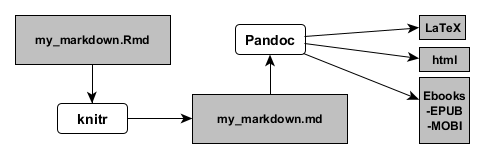
\includegraphics[width=0.6\linewidth]{img/BookdownProc} 

}

\caption{Tulostiedoston prosessointi}\label{fig:L3bdprocess1}
\end{figure}

  \bibliography{jhca2020.bib,packages.bib}

\end{document}
